% Paquets généraux
\documentclass[a4paper,12pt,titlepage,twoside]{article}
\usepackage[T1]{fontenc}
\usepackage[utf8]{inputenc}
\usepackage[french]{babel}
\addto\captionsfrench{%
  \renewcommand{\tablename}{Tableau}%
}
\usepackage[gen]{eurosym}
%\usepackage[dvips]{graphicx}
\usepackage{fancyhdr}
\usepackage{pdfpages} 
\usepackage{multido}
\usepackage{hyperref}
%\usepackage{textcomp}
\usepackage{schemabloc}
\usepackage[bitstream-charter]{mathdesign}
\usepackage{array}
\newcolumntype{P}[1]{>{\centering\arraybackslash}p{#1}}

\newcommand{\id}{54}
\newcommand{\nom}{Liaisons mécaniques}
\newcommand{\sequence}{04}
\newcommand{\num}{01}
\newcommand{\type}{TP}
\newcommand{\descrip}{Modélisation d'un solide. Comportement des liaisons mécaniques. Modéliser les mécanismes du laboratoire par un schéma cinématique, paramétré.}
\newcommand{\competences}{A3-C4: Analyse d'architecture et de comportement \\ &  Mod1-C1: Isolement d'un solide ou d'un système de solides \\ &  Mod2-C10-1: Modèle de solide indéformable \\ &  Mod2-C11: Modélisation géométrique et cinématique des mouvements entre solides indéformables \\ &  Mod2-C12: Modélisation cinématique des liaisons entre solides \\ &  Mod2-C15: Modélisation des actions mécaniques \\ &  Rés-C6: Utilisation d'un solveur ou d'un logiciel multi physique \\ &  Com1-C1: Différents descripteurs introduits dans le programme \\ &  Com2-C4: Outils de communication}
\newcommand{\nbcomp}{9}
\newcommand{\systemes}{Plateforme Stewart}
\newcommand{\systemessansaccent}{Plateforme Stewart}
\newcommand{\ilot}{2}
\newcommand{\ilotstr}{02}
\newcommand{\dossierilot}{\detokenize{Ilot_02 Plateforme Stewart}}
\newcommand{\imageun}{Plateforme}

\newcommand{\urlsysteme}{\href{https://www.costadoat.fr/systeme/57}{Ressources système}}
\newcommand{\matlabsimscape}{\href{https://github.com/Costadoat/Sciences-Ingenieur/raw/master/Systemes/Plateforme Stewart/Plateforme_Stewart_Simscape.zip}{Modèle Simscape}}
\newcommand{\solidworks}{\href{https://github.com/Costadoat/Sciences-Ingenieur/raw/master/Systemes/Plateforme Stewart/Plateforme_Stewart_Solidworks.zip}{Modèle Solidworks}}
\newcommand{\edrawings}{\href{https://github.com/Costadoat/Sciences-Ingenieur/raw/master/Systemes/Plateforme Stewart/Plateforme_Stewart.EASM}{Modèle eDrawings}}
\newcommand{\test}{Stewart_param1}
\newcommand{\testi}{Stewart_param2}
\newcommand{\testii}{Stewart_param3}
\newcommand{\testiii}{Stewart_param4}
\newcommand{\testiiii}{Stewart_euler}


\newcommand{\institute}{Lycée Dorian}


\usepackage{color}
\usepackage{xcolor}
\usepackage{colortbl}
\usepackage{helvet}
\renewcommand{\familydefault}{\sfdefault}
\usepackage{amsfonts}
\usepackage{amsmath}
%\usepackage{xspace}
\usepackage{varioref}
\usepackage{tabularx}
%\usepackage{floatflt}
\usepackage{graphics}
\usepackage{wrapfig}
\usepackage{textcomp}
\usepackage{tikz}
\usepackage{wrapfig}
\usepackage{gensymb}
\usepackage[percent]{overpic}
\usepackage[european]{circuitikz}
\usetikzlibrary{babel}
\usepackage{ifthen}
\usepackage{cancel}
\usepackage{etoolbox}
\usepackage{multirow}
%\usepackage{boxedminipage}
\definecolor{gris25}{gray}{0.75}
\definecolor{bleu}{RGB}{18,33,98}
\definecolor{bleuf}{RGB}{42,94,171}
\definecolor{bleuc}{RGB}{231,239,247}
\definecolor{rougef}{RGB}{185,18,27}
\definecolor{rougec}{RGB}{255,188,204}%255,230,231
\definecolor{vertf}{RGB}{103,126,82}
\definecolor{vertc}{RGB}{220,255,191}
\definecolor{forestgreen}{rgb}{0.13,0.54,0.13}
\definecolor{blcr}{rgb}{0.59,0.69,0.84}
\definecolor{blfr}{rgb}{0.32,0.51,0.75}
\definecolor{orfr}{rgb}{0.90,0.42,0.15}
\definecolor{orcr}{rgb}{0.90,0.65,0.50}
\definecolor{orangef}{rgb}{0.659,0.269,0.072}
\definecolor{orange}{rgb}{0.58,0.35,0.063}
\definecolor{orangec}{rgb}{0.43,0.32,0.25}
\definecolor{rcorrect}{rgb}{0.6,0,0}
\definecolor{sequence}{rgb}{0.75,0.75,0.75}
\definecolor{competences}{rgb}{0.61,0.73,0.35}
\definecolor{grisf}{HTML}{222222}
\definecolor{grisc}{HTML}{636363}
\definecolor{normal}{HTML}{4087c4}
\definecolor{info}{HTML}{5bc0de}
\definecolor{success}{RGB}{92,184,92}
\definecolor{warning}{RGB}{240,173,78}
\definecolor{danger}{RGB}{217,83,79}
\hypersetup{                    % parametrage des hyperliens
    colorlinks=true,                % colorise les liens
    breaklinks=true,                % permet les retours à la ligne pour les liens trop longs
    urlcolor= blfr,                 % couleur des hyperliens
    linkcolor= orange,                % couleur des liens internes aux documents (index, figures, tableaux, equations,...)
    citecolor= forestgreen                % couleur des liens vers les references bibliographiques
    }

% Mise en page
\pagestyle{fancy}

\setlength{\hoffset}{-18pt}
\setlength{\oddsidemargin}{0pt} 	% Marge gauche sur pages impaire2s
\setlength{\evensidemargin}{0pt} 	% Marge gauche sur pages paires
\setlength{\marginparwidth}{00pt} 	% Largeur de note dans la marge
\setlength{\headwidth}{481pt} 	 	% Largeur de la zone de tête (17cm)
\setlength{\textwidth}{481pt} 	 	% Largeu\textbf{r de la zone de texte (17cm)
\setlength{\voffset}{-18pt} 		% Bon pour DOS
\setlength{\marginparsep}{7pt}	 	% Séparation de la marge
\setlength{\topmargin}{-30pt} 		% Pas de marge en haut
\setlength{\headheight}{55pt} 		% Haut de page
\setlength{\headsep}{20pt} 		% Entre le haut de page et le texte
\setlength{\footskip}{30pt} 		% Bas de\textbf{ page + séparation
\setlength{\textheight}{700pt} 		% Hauteur de l'icone zone de texte (25cm)
\setlength\fboxrule{1 pt}
\renewcommand{\baselinestretch}{1}
\setcounter{tocdepth}{1}
\newcommand{\cadre}[2]
{\fbox{
  \begin{minipage}{#1\linewidth}
   \begin{center}
    #2\\
   \end{center}
  \end{minipage}
 }
}

\newcommand{\repon}[1]
{
~\ \\
\begin{tabular}{|m{\linewidth}|}
 \hline
\multido{}{#1}{\\ \hline}
\end{tabular}
}

\newcounter{num_quest} \setcounter{num_quest}{0}
\newcounter{num_rep} \setcounter{num_rep}{0}
\newcounter{num_cor} \setcounter{num_cor}{0}

\newcommand{\question}[1]{\refstepcounter{num_quest}\par
~\ \\ \parbox[t][][t]{0.15\linewidth}{\textbf{Question \arabic{num_quest}}}\parbox[t][][t]{0.85\linewidth}{#1}\par
}


\newcommand{\reponse}[1]
{\refstepcounter{num_rep}
\noindent
\rule{\linewidth}{.5pt}
\textbf{Question \arabic{num_rep}:}
\multido{\i=1+1}{#1}{~\ \\}
}

\newcommand{\cor}
{\refstepcounter{num_cor}
\noindent
\rule{\linewidth}{.5pt}
\textbf{Question \arabic{num_cor}:} \\
}

\newcommand{\repcarre}[2]
{
~\ \\
\begin{tikzpicture}
\draw [fill=white] (0,0) rectangle +(\linewidth,#1);
\node[align=left] at (1.1,#2-0.3) {\textbf{Question #1:}};
\end{tikzpicture}
}

\newcommand{\titre}[1]
{\begin{center}
\cadre{0.8}{\huge #1} 
\end{center}
}


% En tête et pied de page
\lhead{\nom}
\rhead{
\includegraphics[width=2cm]{../../../../img/logo}}
\lfoot{\auteurun,\ \auteurdeux}
\cfoot{Page \thepage}

\fancypagestyle{documentreponse}{%
  \fancyhf{}
  \fancyhead[LO]{Nom: ........................ Prénom: ........................}
  \fancyhead[LE]{\nom}
  \fancyhead[RE,RO]{
\includegraphics[width=2cm]{../../../../img/logo}}
  \lfoot{Document réponse}
  \cfoot{Page \thepage}
   }
  
\fancypagestyle{correction}{%
  \fancyhf{}
  \lhead{\colorbox{danger}{\begin{minipage}{0.65\paperwidth} \textcolor{white}{\textbf{Correction}} \end{minipage}} }
  \rhead{
\includegraphics[width=2cm]{../../../../img/logo}}
  \lfoot{Renaud Costadoat, Françoise Puig}
  \rfoot{\colorbox{danger}{\begin{minipage}{0.5\paperwidth} \begin{flushright}\textcolor{white}{\textbf{Correction}}\end{flushright} \end{minipage}} }}

\fancypagestyle{correctioninfo}{%
  \fancyhf{}
  \lhead{\colorbox{danger}{\begin{minipage}{0.65\paperwidth} \textcolor{white}{\textbf{Correction}} \end{minipage}} }
  \rhead{
\includegraphics[width=2cm]{../../../../img/logo}}
  \lfoot{Renaud Costadoat, Juliette Genzmer, Willie Robert}
  \rfoot{\colorbox{danger}{\begin{minipage}{0.6\paperwidth} \begin{flushright}\textcolor{white}{\textbf{Correction}}\end{flushright} \end{minipage}} }}

\renewcommand{\footrulewidth}{0.4pt}

\usepackage{eso-pic}
\newcommand{\BackgroundPic}{%
\put(0,0){%
\parbox[b][\paperheight]{\paperwidth}{%
\vfill
\begin{center}
\hspace{0.5cm}\vspace{0.5cm}

\includegraphics[width=\paperwidth,height=\paperheight,%
keepaspectratio]{../../../../img/fond3}%
\end{center}
\vfill
}}}

\newcommand{\BackgroundPicdeux}{%
\put(25,-30){%
\parbox[b][\paperheight]{\paperwidth}{%
\vfill
\begin{center}
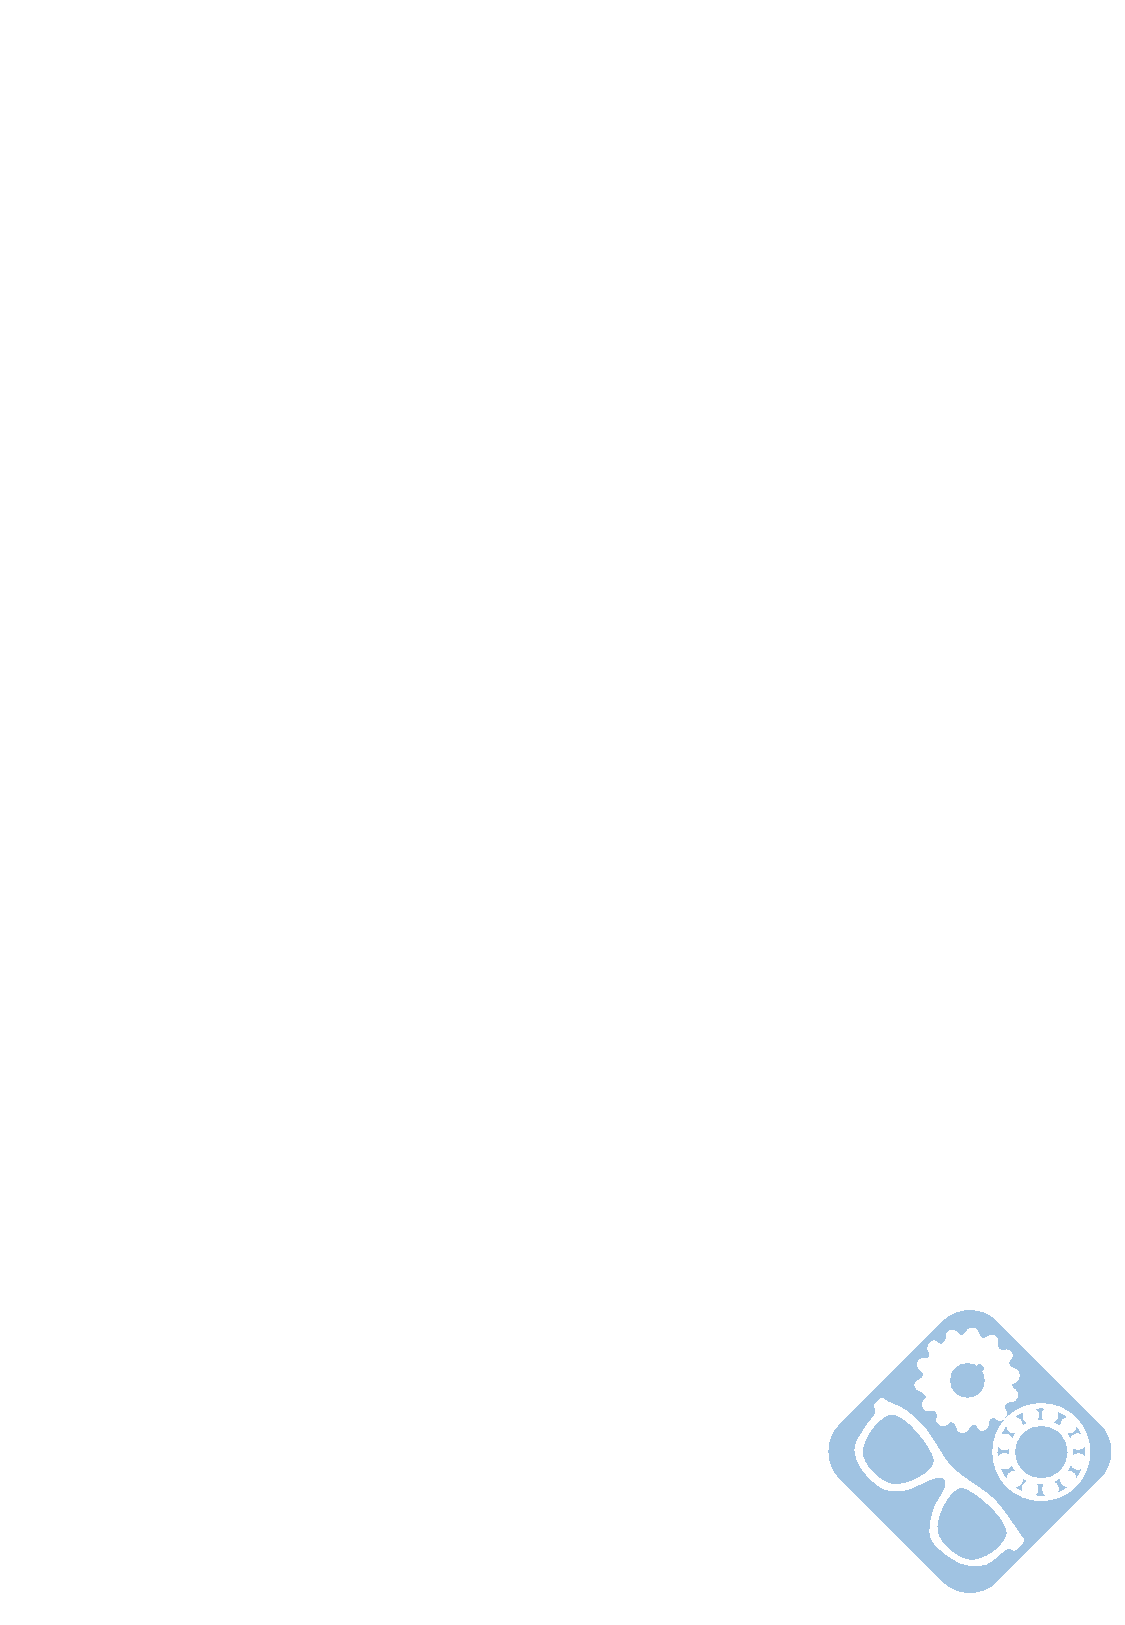
\includegraphics[width=\paperwidth,height=\paperheight,%
keepaspectratio]{../../../../img/fond4}%
\end{center}
\vfill
}}}

\begin{document}

\pagestyle{empty}

\AddToShipoutPicture*{\BackgroundPic}


\includegraphics[width=2cm]{../../../../img/logo}

\Huge{DS \num\ - \sujet}

\vspace{1cm}

\ifdef{\prive}{\begin{center}\colorbox{danger}{\Huge{Avec Correction}}\end{center}}{}

\begin{center}
\centering\huge{PTSI}
\end{center}

\vspace{2cm}


\begin{center}
\centering\Large{\jour}
\end{center}

\vspace{2cm}

\normalsize

\tableofcontents

\newpage

\AddToShipoutPicture{\BackgroundPicdeux}

\pagestyle{fancy}

\begin{center}
\Huge \sujet
\end{center}


\normalsize

\section{Contexte et étude préliminaire}

\begin{figure}[!h]
 \centering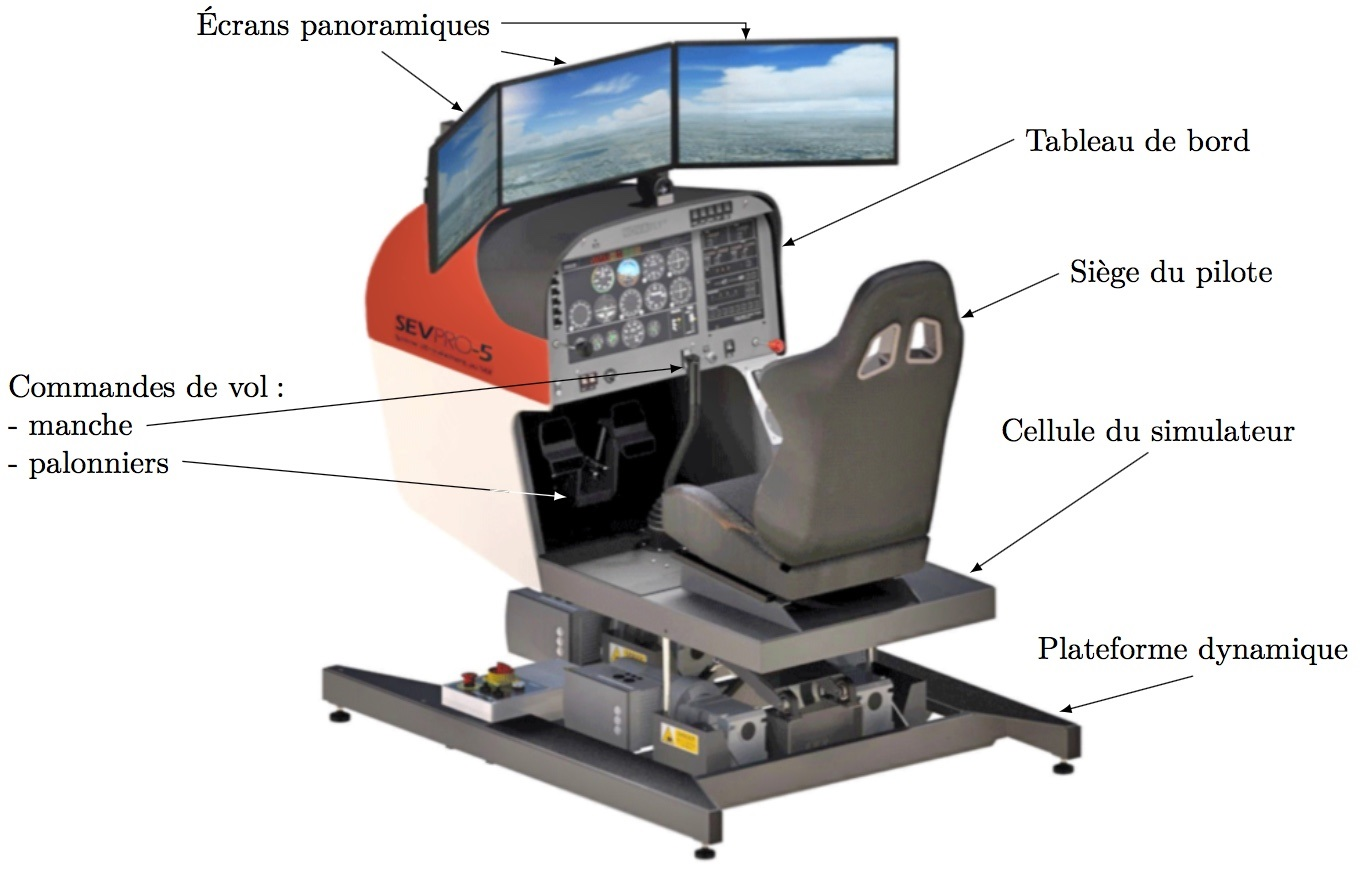
\includegraphics[width=0.7\linewidth]{img/figure_1}
 \caption{Simulateur de vol à plateforme dynamique}
 \label{img01}
\end{figure}

\paragraph{Objectif}

Vérifier la pertinence économique de l'utilisation d'un simulateur de vol pour la formation des pilotes. 

Selon les informations de la Fédération Française Aéronautique (FFA), il y a actuellement près de 47000 pilotes licenciés répartis dans 600 aéroclubs et environ 8000 pilotes nouvellement formés chaque année au plan national. Toutefois, la FFA cherche à augmenter le nombre de licenciés afin d'améliorer son développement et de continuer à promouvoir les activités aéronautiques.

Dans les aéroclubs français, chaque année, la formation des nouveaux pilotes est validée par deux certifications :\begin{itemize}
 \item le Brevet de Base (BB) qui permet de voler seul à bord d'un aéronef, au voisinage de l'aérodrome de départ ;
 \item la licence de pilote privé, PPL (Private Pilot Licence), titre européen qui autorise à voler dans des conditions météorologiques permettant le vol à vue. La license PPL permet de voyager avec des passagers, sans limitation de distance et sous réserve que cela ne constitue pas une activité lucrative.
\end{itemize}

En complément d'une formation théorique spécifique, il faut avoir accompli 45 heures de vol, avec un minimum de 25 heures de vol en double commande (avec instructeur dans l'avion) et au moins 10 heures de vol en solo supervisé (avec instructeur au sol). Le reste est constitué d'heures de vol en solo (sans instructeur). Actuellement, sur les 45 heures de vol nécessaires pour la formation PPL, 5 heures de simulateur au maximum peuvent être officiellement validées comme des heures de vol en solo sur avion réel, sous réserve qu'elles soient effectuées en présence d'un instructeur et sur un simulateur de vol certifié comme celui de la figure 
\ref{img01}. 

La formation en vol traditionnelle se fait sur des avions fiables et économiques tels que le Robin DR400 (figure \ref{img04}). 

\begin{figure}[!h]
 \centering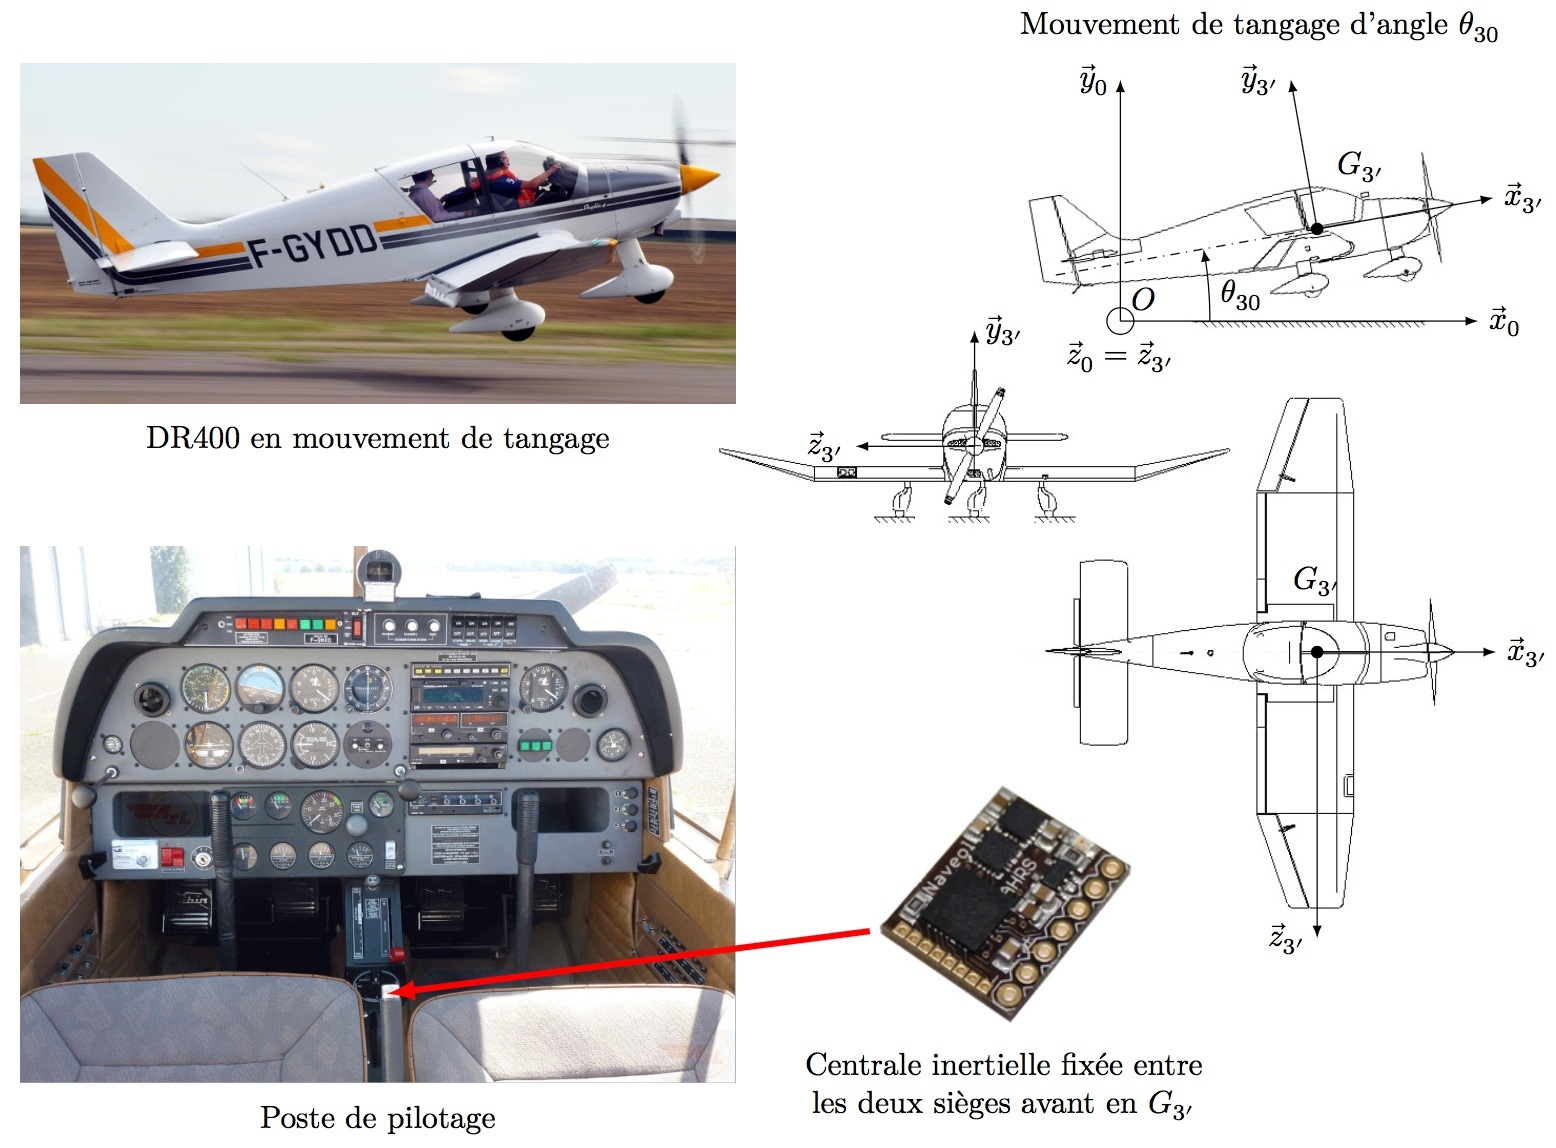
\includegraphics[width=0.7\linewidth]{img/figure_4}
 \caption{Paramétrage du mouvement de tangage d'un DR400}
 \label{img04}
\end{figure}

Les tarifs pratiqués pour un vol sur DR400 sont environ de 135 \euro /h en vol solo et de 160 \euro /h avec instructeur à bord ou au sol, carburant inclus. 

Les simulateurs de vol disponibles sur le marché sont constitués de deux ensembles complémentaires : 
\begin{itemize}
 \item la cellule du simulateur de base, dotée d'un ordinateur équipé d'un logiciel de simulation de vol, de trois écrans panoramiques ainsi que des commandes de vol, de type manche et palonniers, avec ou sans retour d'efforts ; 
 \item la plateforme dynamique qui met en mouvement la cellule du simulateur. Commandée par le logiciel de simulation de vol, la plateforme dynamique permet de faire ressentir au pilote des sensations proches de celles du vol à bord d'un avion réel. 
\end{itemize}

Les aéroclubs souhaitent se doter de tels simulateurs afin de diminuer le cout de la formation et aussi d'inciter 
davantage de personnes à se lancer dans l'aventure aéronautique. Il faut prévoir environ 35 \euro /h pour une 
utilisation en solo du simulateur de vol et 60 \euro /h pour une utilisation avec instructeur. 

\begin{figure}[!h]
 \centering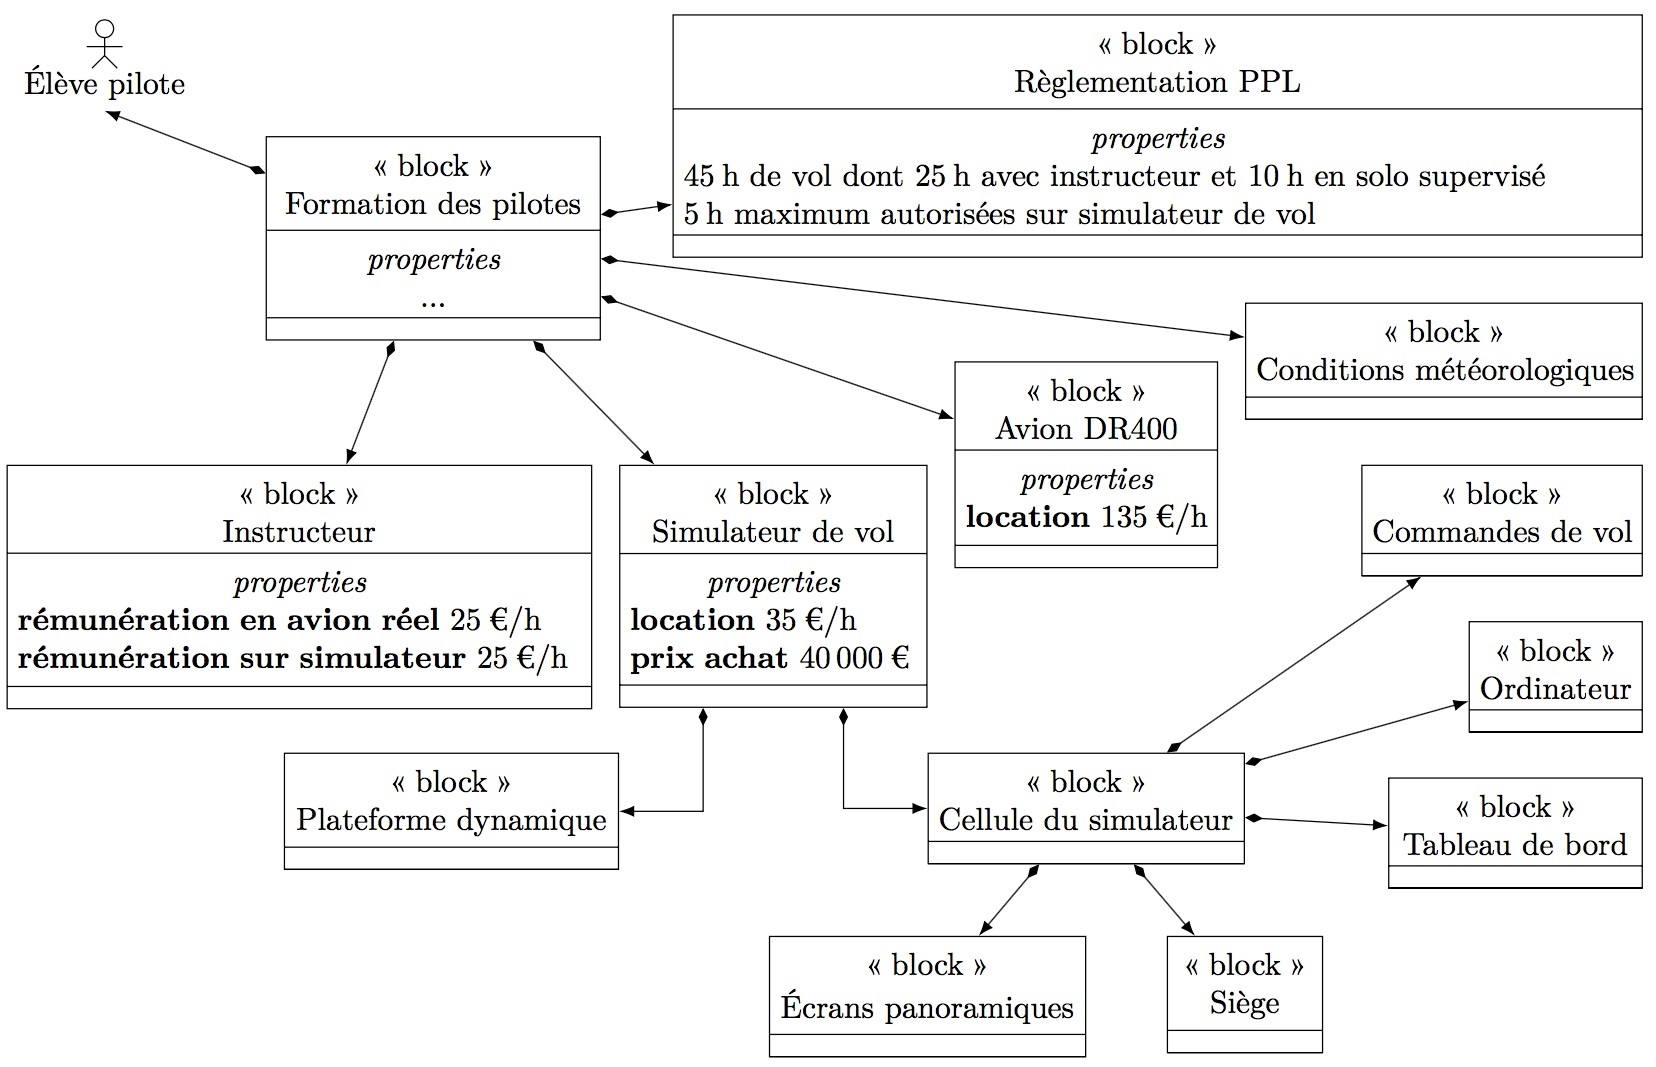
\includegraphics[width=0.9\linewidth]{img/figure_2}
 \caption{Contexte économique de la formation des pilotes}
 \label{img02}
\end{figure}

Certaines phases de la formation telles que l'entrainement au vol sans visibilité ou la compréhension et l'utilisa­tion des instruments de radionavigation sont plus efficaces sur un simulateur que dans un avion réel. En effet, il est plus aisé pour un instructeur de former le pilote sur un simulateur lors de ces phases car il n'y a pas la gène du bruit de l'avion réel et il y a la possibilité de mettre la simulation en pause afin de donner des explications tant sur l'analyse de la situation de vol que sur le comportement à adopter. 
Le rôle du simulateur est ainsi de compléter la formation indépendamment des conditions météorologiques et en toute sécurité. Les aéroclubs dotés de simulateurs de vol peuvent alors avoir une activité de formation tout au long de l'année, quelles que soient les conditions météorologiques. 

\newpage

\begin{figure}[!h]
 \centering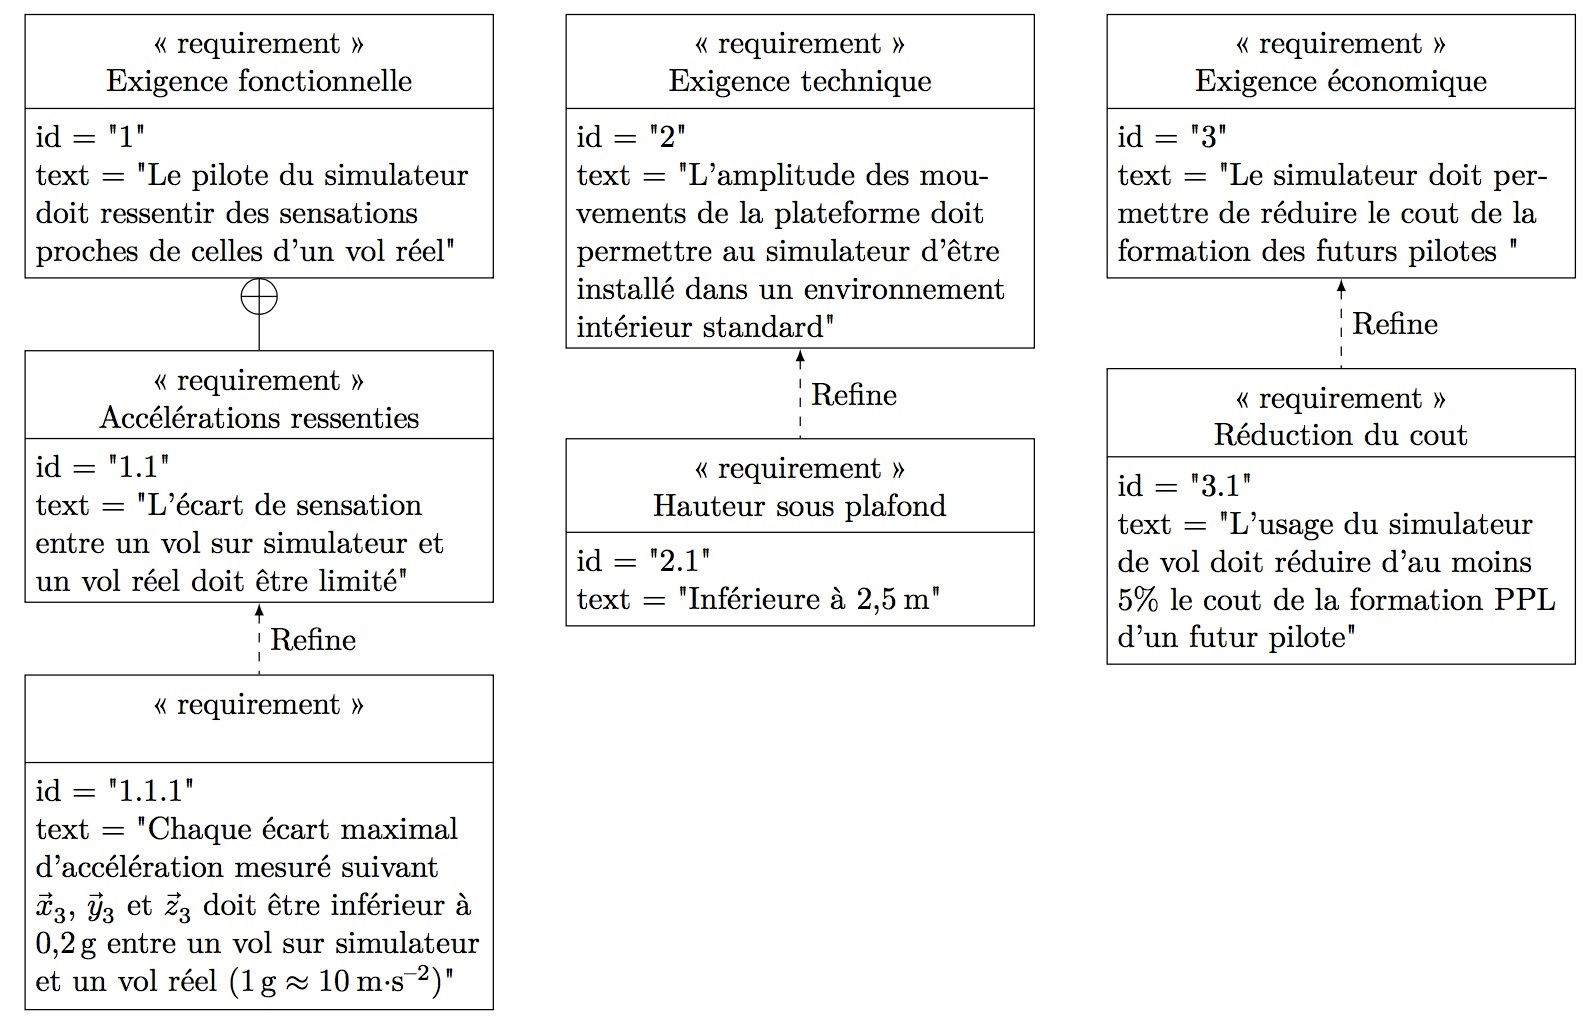
\includegraphics[width=0.9\linewidth]{img/figure_3}
 \caption{Diagramme des exigences partiel du simulateur de vol}
 \label{img03}
\end{figure}

\newpage 

\question{À l'aide des figures \ref{img02} et \ref{img03}:}
\begin{itemize}
 \item calculer le cout minimal de la formation en vol traditionnelle d'un élève pilote pour la licence PPL (c'est-à-­dire uniquement à l'aide de vols en avion réel de type DR400) ;
 \item calculer le cout minimal de la formation multi-modale d'un élève pilote pour la licence PPL (c'est-à-dire à l'aide de vols en avion réel de type DR400 et sur simulateur de vol) ; 
 \item en déduire l'économie substantielle faite par l'élève pilote, exprimée en pourcentage du cout d'une formation uniquement sur avion réel ; 
 \item conclure quant à la pertinence de l'usage du simulateur de vol dans la formation PPL du point de vue de l'économie financière attendue par les futurs nouveaux pilotes et exprimée 
dans les exigences de la figure \ref{img03}.
\end{itemize} 

Le but du simulateur de vol étant d'assurer le ressenti du pilote au travers de la maitrise des accélérations qu'il subit au cours d'un vol, l'objet de ce sujet est de comparer ces accélérations mesurées sur un ROBIN DR400 en vol et celles mesurées sur le simulateur de vol équipé de la plateforme dynamique. Il s'agira alors d'étudier la minimisation de l'écart entre ces accélérations mesurées entre un vol réel et un vol simulé, tout en respectant les exigences géométriques et économiques des aéroclubs qui sont partiellement exprimées sur la figure \ref{img03}. 

\section{Architecture et conception de la plateforme dynamique}

\paragraph{Objectif}

Déterminer les paramètres angulaires à imposer afin d'obtenir un mouvement de tangage seul du simulateur de vol, puis justifier l'utilisation de vérins à gaz et de réducteurs irréversibles au sein de la plateforme dynamique.

La plateforme dynamique (figure \ref{imgA}) permet de mouvoir la cellule du simulateur (3). Elle est composée de trois servomoteurs identiques qui sont constitués d'une machine électrique, d'un codeur incrémental et d'un variateur de vitesse intégré (figure \ref{imgB}).
%Afin d'améliorer la compacité du système ainsi que son entretien, le constructeur a choisi d'utiliser des machines synchrones pour les chaines de motorisation. Les machines synchrones utilisées sont à aimants permanents et à stators bobinés.
Chaque machine électrique entraine un réducteur de type roue et vis sans fin irréversible, qui transmet l'énergie à un dispositif bielle-manivelle. Chacune des trois bielles est reliée à la cellule du simulateur (3) par un guidage sphérique. \\
La cellule du simulateur (3) est reliée à un bras oscillant (6) par l'intermédiaire d'un joint de Cardan. Le bras oscillant (6) est relié au bâti (0) à l'aide d'une liaison modélisable par une liaison pivot d'axe (E, $\overrightarrow{z_0}$). Deux vérins à gaz {corps (8) + tige (9)} relient le bras oscillant (6) au bâti afin de compenser les effets de la gravité et faciliter l'action des motorisations.\\
Sur le modèle plan de la figure \ref{imgC}, les deux vérins à gaz sont modélisés par une seule liaison glissière de direction $\overrightarrow{y_{89}}$ entre la tige (9) et le corps (8), ainsi qu'un ressort de compression (non représenté) entre ces deux mêmes solides, qui exerce un effort sur (8) et sur (9).

Les liaisons et paramètres géométriques sont les suivants (figures \ref{imgA} et \ref{imgC}) :
\begin{itemize}
 \item la liaison pivot d'axe (E, $\overrightarrow{z_0}=\overrightarrow{z_6}$) entre le bras oscillant (6) et le bâti (0) est paramétrée par l'angle $\theta_{60}=(\overrightarrow{x_0},\overrightarrow{x_6})=(\overrightarrow{y_0},\overrightarrow{y_6})$,
 \item $\overrightarrow{EC}=L.\overrightarrow{x_6}$,
 \item le joint de Cardan entre la cellule du simulateur (3) et le bras oscillant (6) est modélisable par une liaison sphérique à doigt de centre C, interdisant la rotation autour de (C, $\overrightarrow{y_3}$). Les mouvements de (3) par rapport à (6) sont paramétrés par les angles $\theta_{x36}$ et $\theta_{z36}$ comme indiqué sur la figure \ref{img08}.
\end{itemize}

\begin{figure}[!h]
 \centering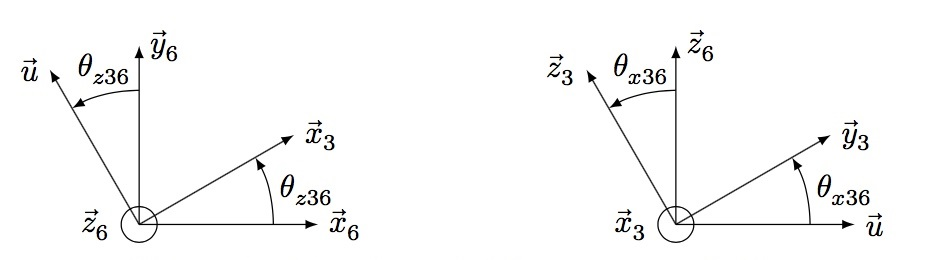
\includegraphics[width=0.7\linewidth]{img/figure_8}
 \caption{Rotations de (3) par rapport à (6)}
 \label{img08}
\end{figure}

\subsection{Analyse des paramètres à imposer pour obtenir un mouvement de tangage seul du simulateur}

\question{Exprimer, en projection dans la base $R_3(\overrightarrow{x_3},\overrightarrow{y_3})$, le vecteur vitesse de rotation du mouvement de (3) par rapport à (0) en fonction de $\dot{\theta}_{60}$, $\dot{\theta}_{x36}$ et $\dot{\theta}_{z36}$.}

\question{Déterminer les paramètres angulaires à imposer afin d'obtenir un mouvement de tangage seul du simulateur de vol} ~\ \\

Les deux vérins à gaz se comportent comme des ressorts de compression et ont pour fonction de positionner
verticalement le point C de la cellule du simulateur (3) à une position d'équilibre moyenne définie par l'angle
$\theta_{60moy}$, lorsque les biellettes (2), (4) et (4bis) ne sont pas liées respectivement aux manivelles (1), (5) et (5bis).

Dans cette situation $\theta_{30}=0°$ et $\overrightarrow{G_3C}$ est vertical.

\begin{figure}[!h]
 \centering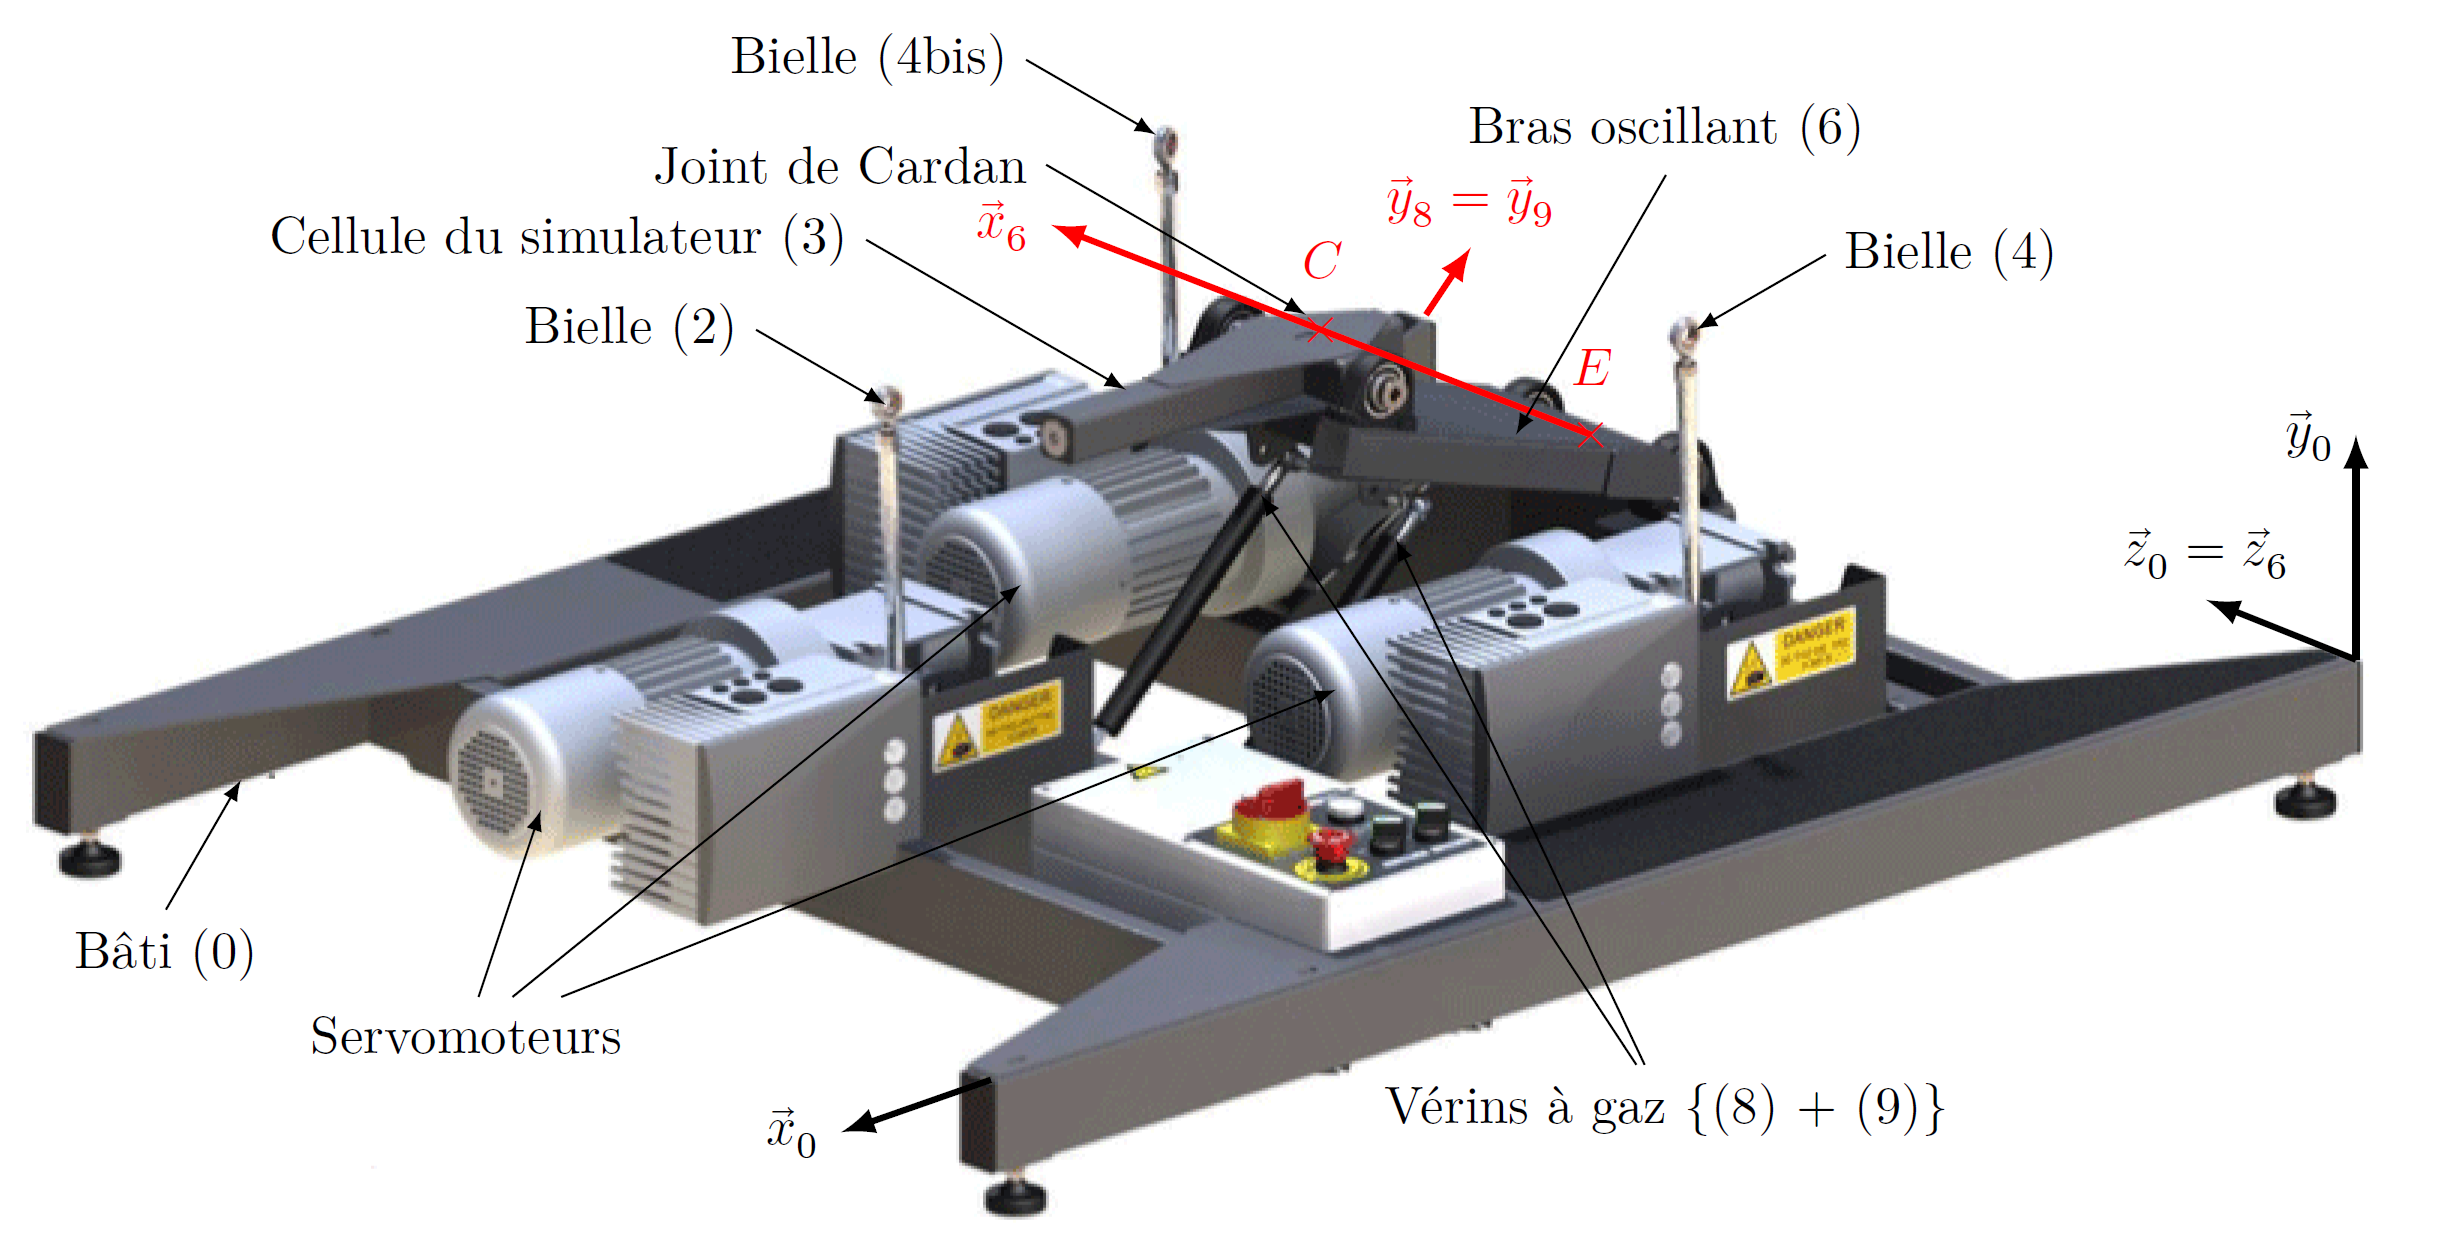
\includegraphics[width=0.8\linewidth]{img/figure_A}
 \caption{Plateforme dynamique}
 \label{imgA}
\end{figure}

\begin{figure}[!h]
 \centering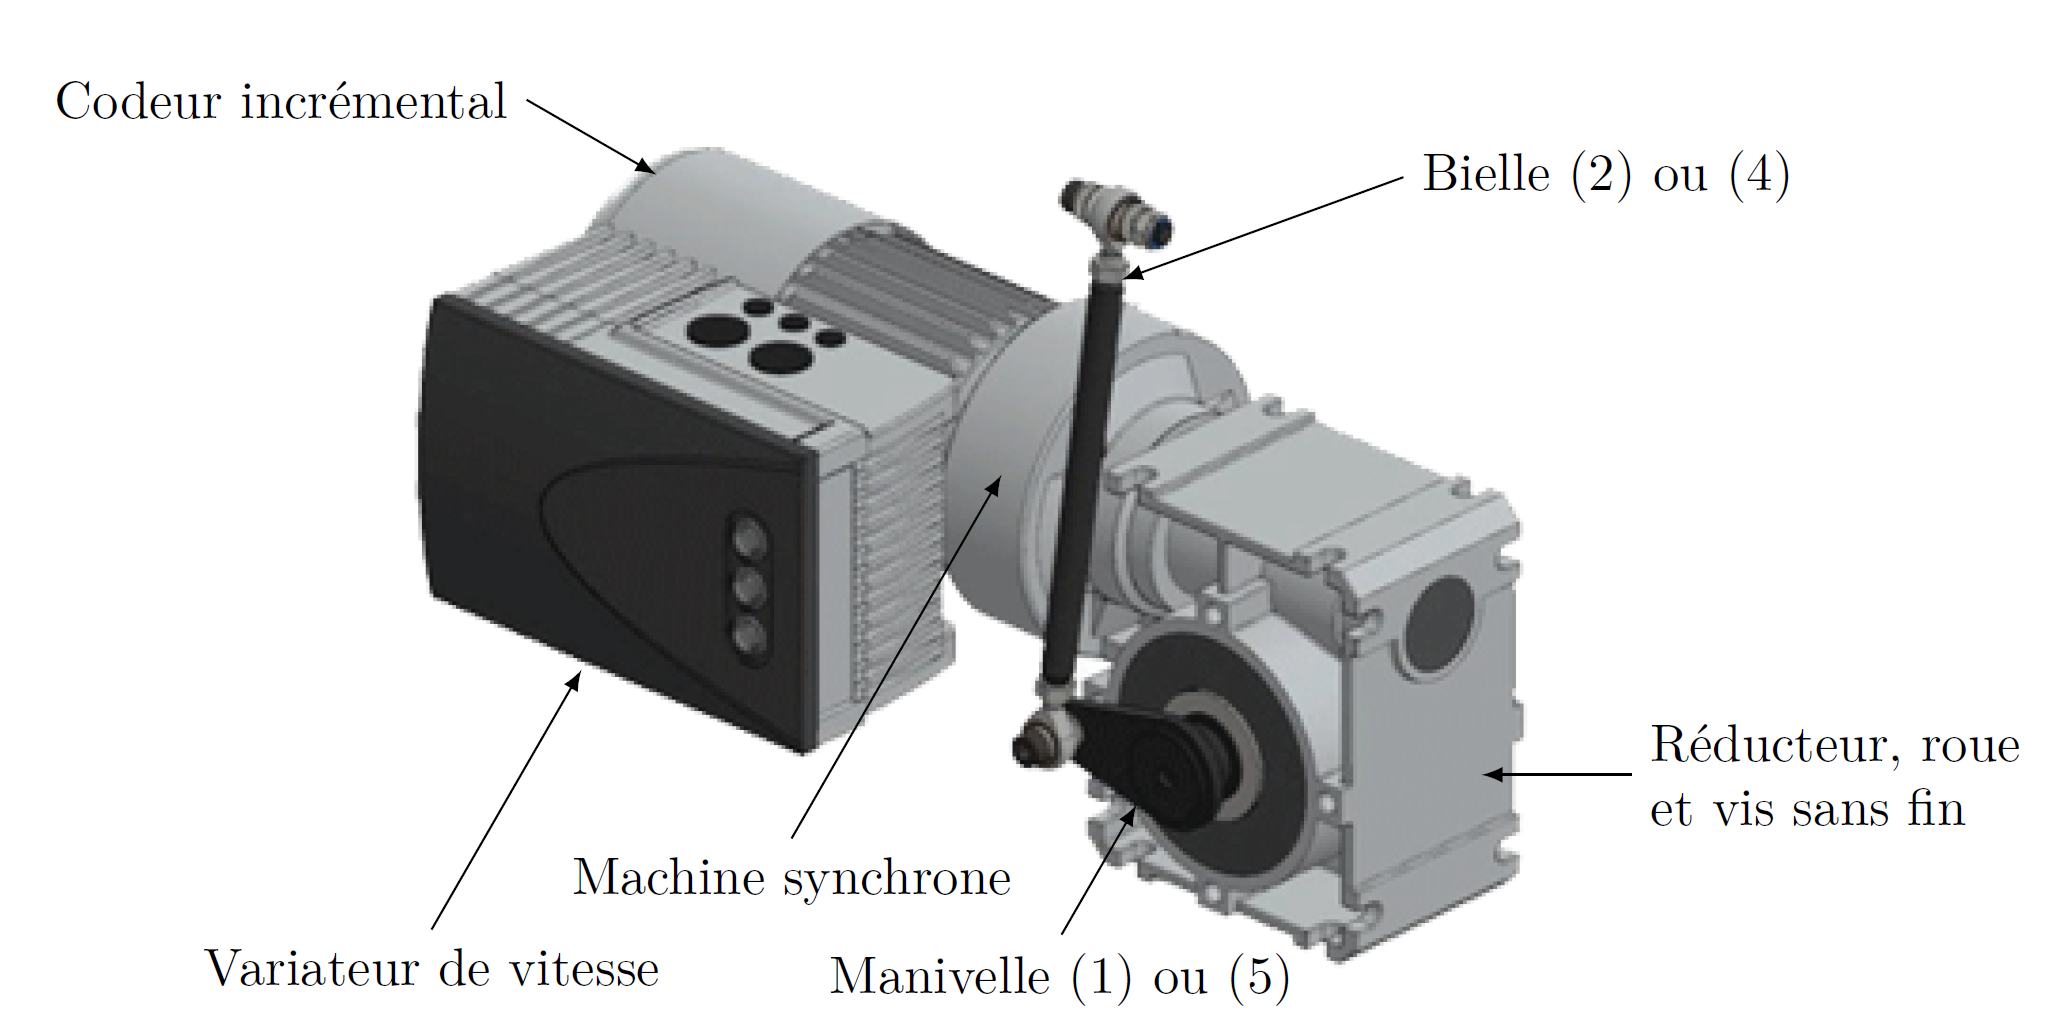
\includegraphics[width=0.7\linewidth]{img/figure_B}
 \caption{Servomoteur}
 \label{imgB}
\end{figure}

\newpage

\begin{figure}[!h]
 \centering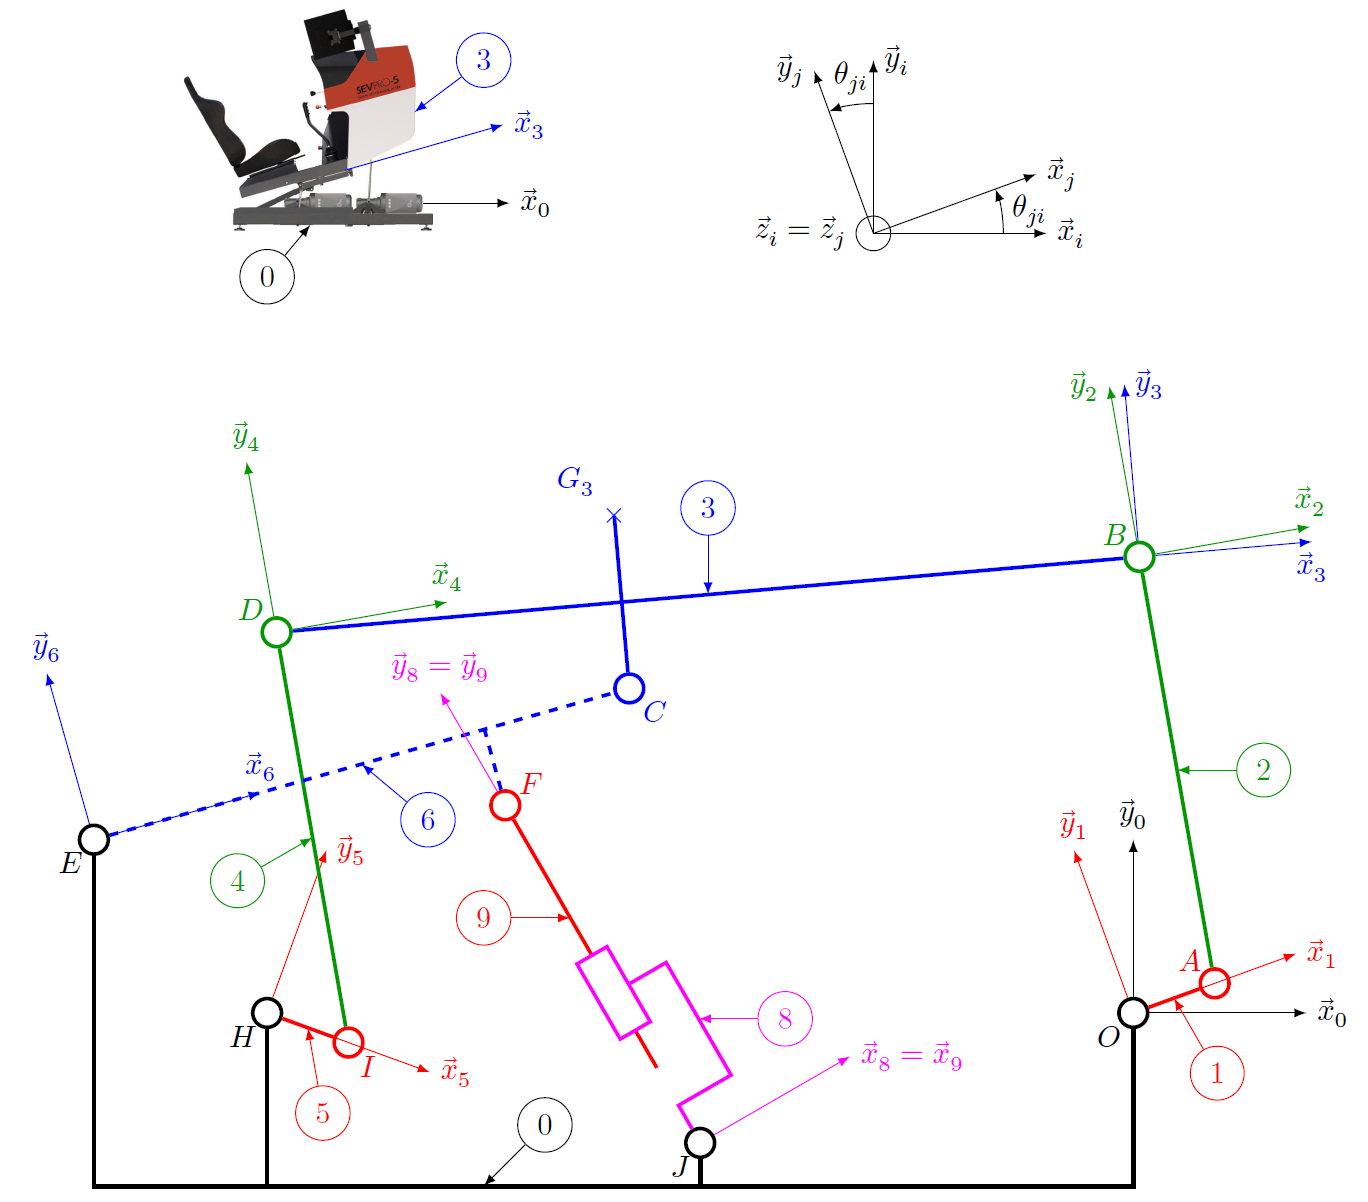
\includegraphics[width=0.9\linewidth]{img/figure_C}
 \caption{Schéma cinématique de la plateforme dynamique en modélisation plane dans le plan (O, $\protect\overrightarrow{x_0}$, $\protect\overrightarrow{y_0}$)}
 \label{imgC}
\end{figure}

\begin{figure}[!h]
 \centering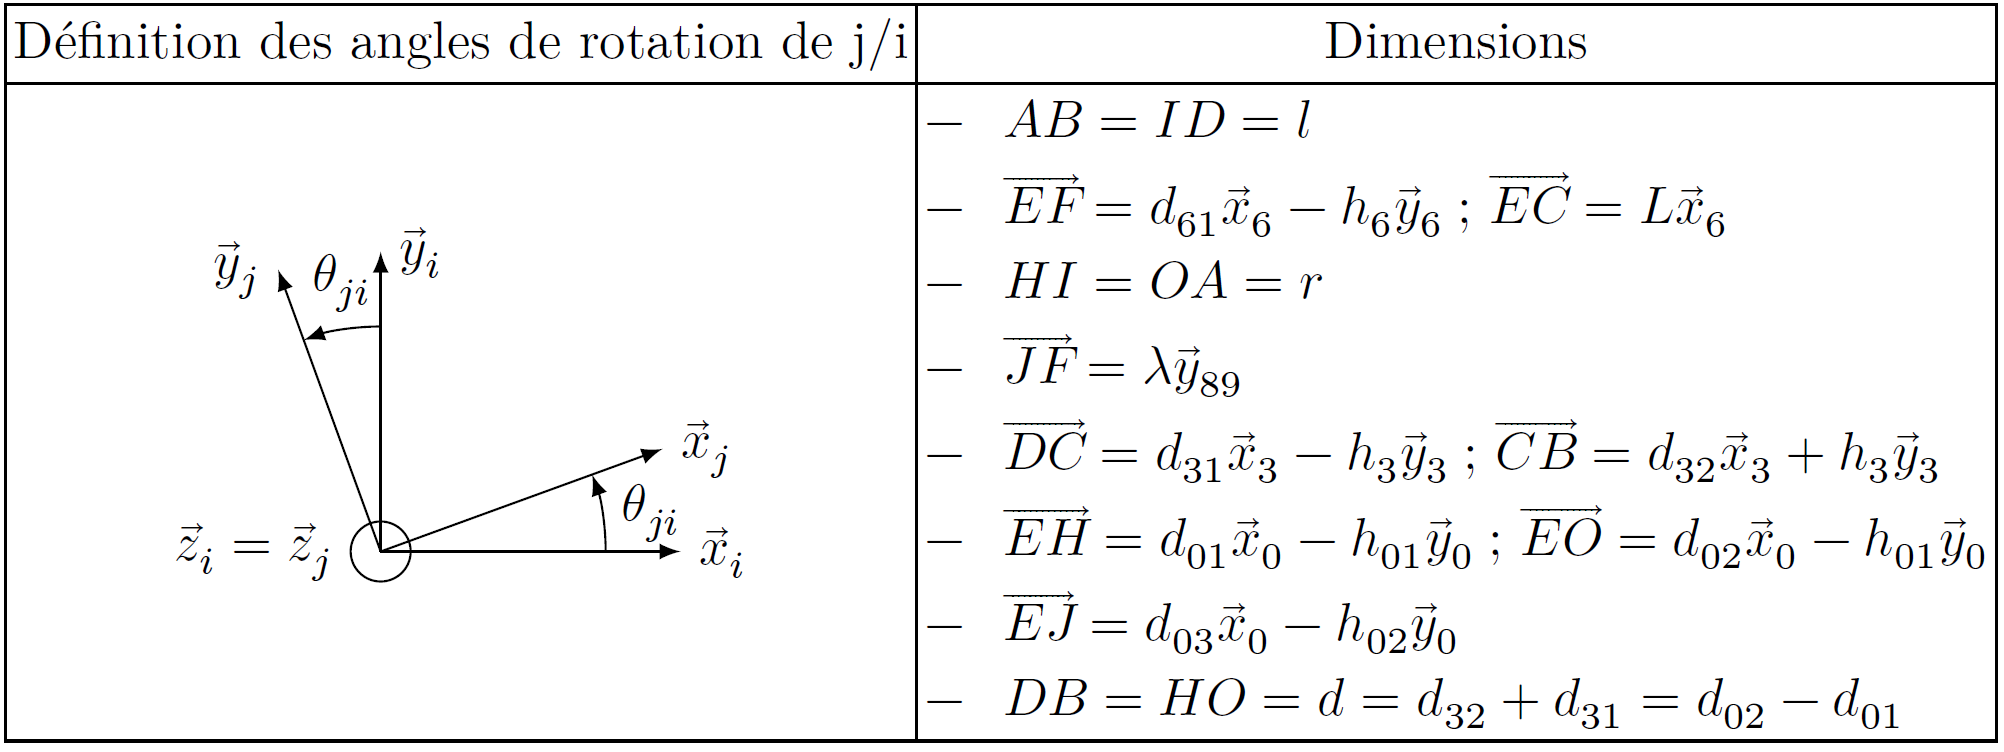
\includegraphics[width=0.7\linewidth]{img/figure_D}
 \caption{Repérage et paramétrage du mouvement de tangage}
 \label{imgD}
\end{figure}

\newpage

\section{Commande d'un mouvement de tangage du simulateur de vol}

\subsection{Modélisation du comportement de la chaine cinématique}


\paragraph{Objectif} Déterminer la loi entrée/sortie de la chaine cinématique de la plateforme dynamique.

\question{Ecrire la fermeture géométrique (vectorielle) de la chaîne OABCEO.}

\question{Projeter cette équation sur $\vec{x_0}$ et $\vec{y_0}$ et écrire les 2 équations trouvées.\label{q1}}

\question{Ecrire la fermeture géométrique (vectorielle) de la chaîne HIDCEH.}

\question{Projeter cette équation sur $\vec{x_0}$ et $\vec{y_0}$ et écrire les 2 équations trouvées.\label{q2}}

\question{A partir des équations trouvées aux question \ref{q1} et \ref{q2}, montrer qu'il est possible d'obtenir les deux équations suivantes :}

\begin{eqnarray}
\lambda_1.(cos\theta_{50}-cos\theta_{10})-\lambda_2.(sin\theta_{40}-sin\theta_{20})+\lambda_3.(-1+cos\theta_{30})=0\\
\lambda_1.(sin\theta_{50}-sin\theta_{10})+\lambda_2.(cos\theta_{40}-cos\theta_{20})+\lambda_3.sin\theta_{30}	=0
\end{eqnarray}

\question{Exprimer les paramètres $\lambda_1$, $\lambda_2$  et $\lambda_3$ en fonction des longueurs $r$, $l$, et $d=d_{31}+d_{32}=d_{02}-d_{01}$.}

\paragraph{Hypothèses relatives aux dispositifs bielle-manivelle} ~\ \\

On prendra pour la suite $r\ll l$ et $\theta_{20}\approx \theta_{40}$.

De plus, dans le cas d'un mouvement de tangage seul, la commande d'origine des moteurs est telle que $\theta_{10}=-\theta_{50}$ (angles définis sur la figure \ref{imgC}, sur le document réponse) pour pouvoir maximiser les valeurs de l'angle de tangage dans les positions extrêmes des bielles (2) et (4).

\question{En supposant que $r\ll l$, proposer une équation approchées donnant l'expression de $\theta_{30}$ en fonction de $\theta_{10}$ et de paramètres géométriques fournis figure \ref{imgD}.}

\subsection{Étude de la structure de la chaîne cinématique}

\question{Compléter le graphe des liaisons ébauché sur le document réponse.}

\question{Calculer le degré d'hyperstatisme de ce mécanisme. Vous noterez précisément la formule que vous utilisez (méthode cinématique ou méthode statique)}

~\

Le degré d'hyperstatisme de la boucle JFE est $h_{JFE}=3$

\question{Ecrire les torseurs $\left\{V_{8/0}\right\}$, $\left\{V_{8/9}\right\}$, $\left\{V_{9/6}\right\}$ et $\left\{V_{6/0}\right\}$ en utilisant la notation en colonne suivante:}
\begin{center}
$\left\{V_{i/j}\right\}=\left\{\begin{matrix}
 \omega_{xij} & V_{A,xij}  \\ 
 \omega_{yij} & V_{A,yij}  \\ 
 \omega_{zij} & V_{A,zij}  
\end{matrix}
\right\}_{(A,\overset{\scriptscriptstyle \rightharpoonup}{x},\overset{\scriptscriptstyle \rightharpoonup}{y},\overset{\scriptscriptstyle \rightharpoonup}{z})}$
\end{center}

\question{Ecrire la fermeture cinématique à l'aide des torseurs précédents. Après avoir écrit tous les torseurs au point E, en déduire les 6 équations en projection sur $\overrightarrow{x_0}$, $\overrightarrow{y_0}$ et $\overrightarrow{z_0}$.}

\question{Donner les équations qui permettent de retrouver le degré d'hyperstatisme $h_{JFE}$=3}

\question{Quelle(s) modification(s) peut-on apporter pour rendre isostatique cette boucle, sans modifier la liaison 8-9 ?}

\subsection{Modélisation du comportement d'un générateur de consigne en vitesse}

\paragraph{Objectif}

Vérifier la pertinence de la commande en trapèze de vitesse des servomoteurs. \\ ~\

Afin d'éviter des sollicitations mécaniques brutales et dangereuses de la plateforme dynamique, le constructeur a choisi de piloter les moteurs à l'aide de consignes de vitesse de rotation $\omega_{cons}(t)$ de forme trapézoïdale (figure \ref{img11}).

\begin{figure}[!h]
 \centering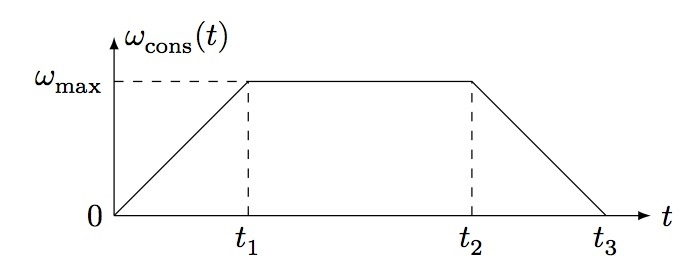
\includegraphics[width=0.7\linewidth]{img/figure_11}
 \caption{Loi en trapèze de vitesse}
 \label{img11}
\end{figure}

\question{En supposant que la vitesse angulaire du moteur $\omega_{m/0}(t)$ (en rad.s$^{-1}$) suive parfaitement l'évolution de la consigne $\omega_{cons}(t)$, déterminer l'expression de la valeur de la position angulaire de l'arbre moteur $\theta_m=\theta_{m/0}$ (en rad) en fonction de $\omega_{max}$, $t_1$, $t_2$ et $t_3$ à partir de la figure \ref{img11}.}

\section{Modélisation du comportement d'un des servomoteurs du simulateur de vol}

\paragraph{Objectif} Proposer un modèle du comportement des servomoteurs du simulateur de vol pour pouvoir ensuite optimiser leurs performances. \\ ~\

Un modèle linéarisé de l'ensemble (Machine synchrone autopilotée + chaine de transmission d'énergie) a été obtenu, dans une étude non présentée ici, en identifiant son comportement à partir d'une simulation numérique
de la zone en pointillés de la figure \ref{img15}. La transformée de Laplace d'une fonction temporelle $f(t)$ est notée $F(p)$.

Comme vu précédemment, la consigne, notée $\omega_{cons}(t)$, est générée sous la forme d'un trapèze de vitesse angulaire de l'arbre moteur analogue à celui de la figure \ref{img11}. Cette consigne de vitesse est ensuite comparée à la vitesse réelle du moteur (machine synchrone) $\omega_{m/0}(t)$, notée à présent $\omega_m(t)$ et mesurée par l'intermédiaire d'un codeur incrémental monté directement sur l'arbre moteur. La sortie du correcteur fournit alors une tension de commande $u_0(t)$ à l'onduleur (pré-actionneur), dont le rôle est de générer trois tensions d'alimentation sinusoïdales déphasées de $\frac{2\pi}{3}$ et d'amplitude $\sqrt{2}.u_0(t)$, notées $v_a(t)$, $v_b(t)$ et $v_c(t)$. Ces tensions alternatives alimentent ensuite la machine synchrone (actionneur) qui convertit l'énergie électrique fournie en énergie mécanique (Remarque : les détails internes des modèles de l'onduleur et de la machine synchrone n'ont volontairement pas été donnés afin de ne pas compliquer inutilement le sujet). Dans le cas du simulateur de vol, les machines synchrones sont autopilotées, c'est-à-dire que la génération électrique des trois tensions alternatives par l'onduleur dépend directement de la position angulaire du rotor et du nombre de paires de pôles de la machine électrique, d'où la boucle d'autopilotage de la figure \ref{img15}. Enfin, $C_r(p)$ correspond au modèle d'un couple résistant rapporté sur l'arbre moteur.

\begin{figure}[!h]
 \centering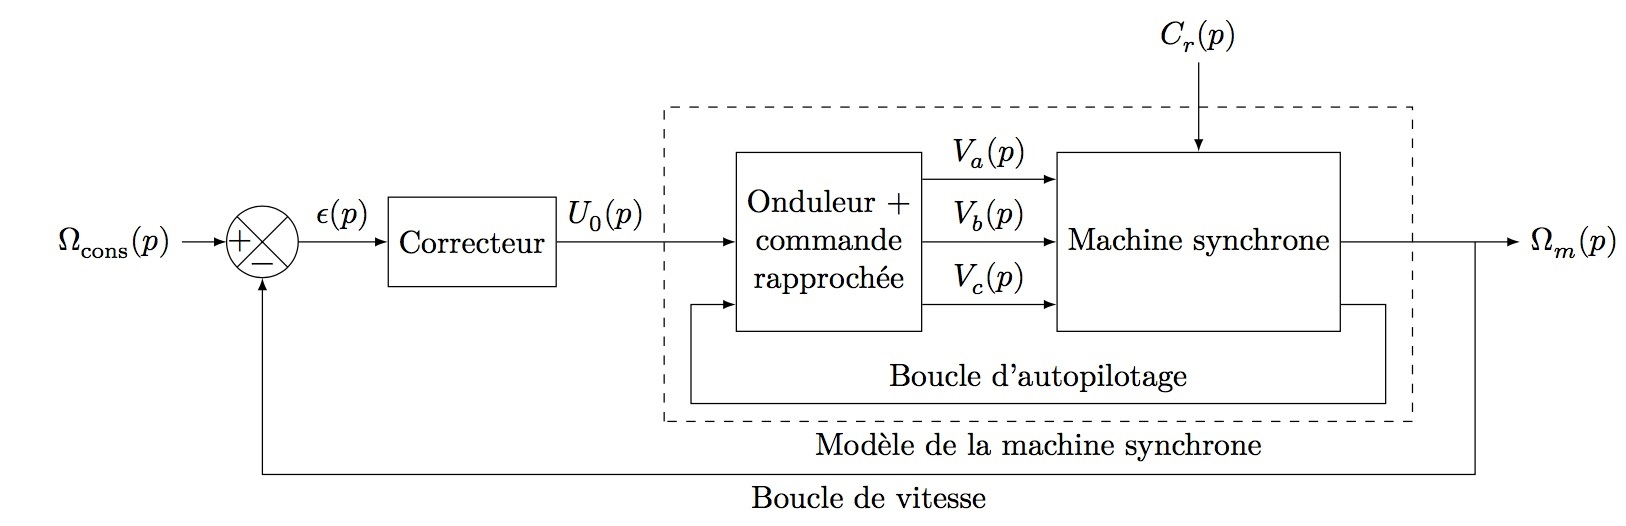
\includegraphics[width=0.7\linewidth]{img/figure_15}
 \caption{Modèle de l'asservissement en vitesse de la machine synchrone autopilotée}
 \label{img15}
\end{figure}

Le problème principal du modèle numérique d'un servomoteur de la figure \ref{img15} est qu'il présente de fortes non-linéarités. En effet, le comportement du modèle dépend de la vitesse angulaire du moteur $\omega_m(t)=\omega_{m/0}(t)$. Pour mettre cela en avant, plusieurs simulations numériques ont été faites pour des vitesses angulaires du moteur $\omega_m(t)$ différentes, un couple résistant $C_r(p)=0$ et la valeur de $J_{eq}$ donnée ($J_{eq}=2,15×10^{-3}$ kg.m$^2$). Pour chacune d'elles, le diagramme de Bode correspondant associé à la fonction de transfert $\left.\frac{\Omega_m(p)}{U_0(p)}\right|_{C_r(p)=0}$ de la machine synchrone autopilotée a été tracé sur la figure \ref{imgE} du document réponse.

Afin d'effectuer le réglage de la loi de commande permettant d'assurer les performances des servomoteurs de
la plateforme dynamique, l'idée consiste à représenter la machine synchrone autopilotée par le modèle de la
figure \ref{img16}, en considérant le cas le plus défavorable possible du point de vue de la stabilité en boucle fermée et des conditions d'utilisation du système.

\question{À partir de tracés effectués sur la figure \ref{imgE} du document réponse, montrer qu'il est possible de mettre $H_{m0}(p)$ sous la forme suivante:}
\begin{center}
$H_{m0}(p)=\frac{K}{1+\frac{2.z}{\omega_0}.p+\frac{1}{\omega_0^2}.p^2}$
\end{center}

\question{Déterminer $H_{m0}(j.\omega_0)$, puis $|H_{m0}(j.\omega_0)|$}

\question{Montrer que $G_{dB}(\omega_0)=20.log(K)-20.log(2.z)$ \label{q3}}

\question{À partir de tracés effectués sur la figure \ref{imgE} du document réponse et du résultat de la question \ref{q3}, proposer un modèle pertinent pour $H_{m0}(p)$, sachant qu'il est souhaité que ce modèle corresponde au comportement de la machine synchrone autopilotée dans le cas le plus défavorable du point de vue de la stabilité en boucle fermée identifié comme celui pour lequel $\omega_m=120$ rad.s$^{-1}$. Écrire la fonction de transfert $H_{m0}(p)$ sous forme canonique en précisant les valeurs numériques de ses paramètres caractéristiques. Les constructions devront apparaître sur les courbes.}

\subsection{Optimisation des performances des servomoteurs}

\paragraph{Objectif} Vérifier que les performances imposées par l'extrait du cahier des charges donné sur le tableau de la figure \ref{img16} sont vérifiées par le modèle d'asservissement de vitesse de la machine synchrone autopilotée et modifier le réglage d'un correcteur le cas échéant.

\question{Déterminer numériquement la fonction de transfert, sous la forme canonique, en boucle fermée non corrigée de l'asservissement de vitesse modélisé sur la figure \ref{img16} avec $H_{cor}(p)=1$, notée $H_{bf\ nc}(p)=\frac{\Omega_m(p)}{\Omega_{cons}(p)}$. Faire l'application numérique.}

\question{Déterminer l'erreur statique et la comparer au cahier des charges.}

\begin{figure}[!h]
 \centering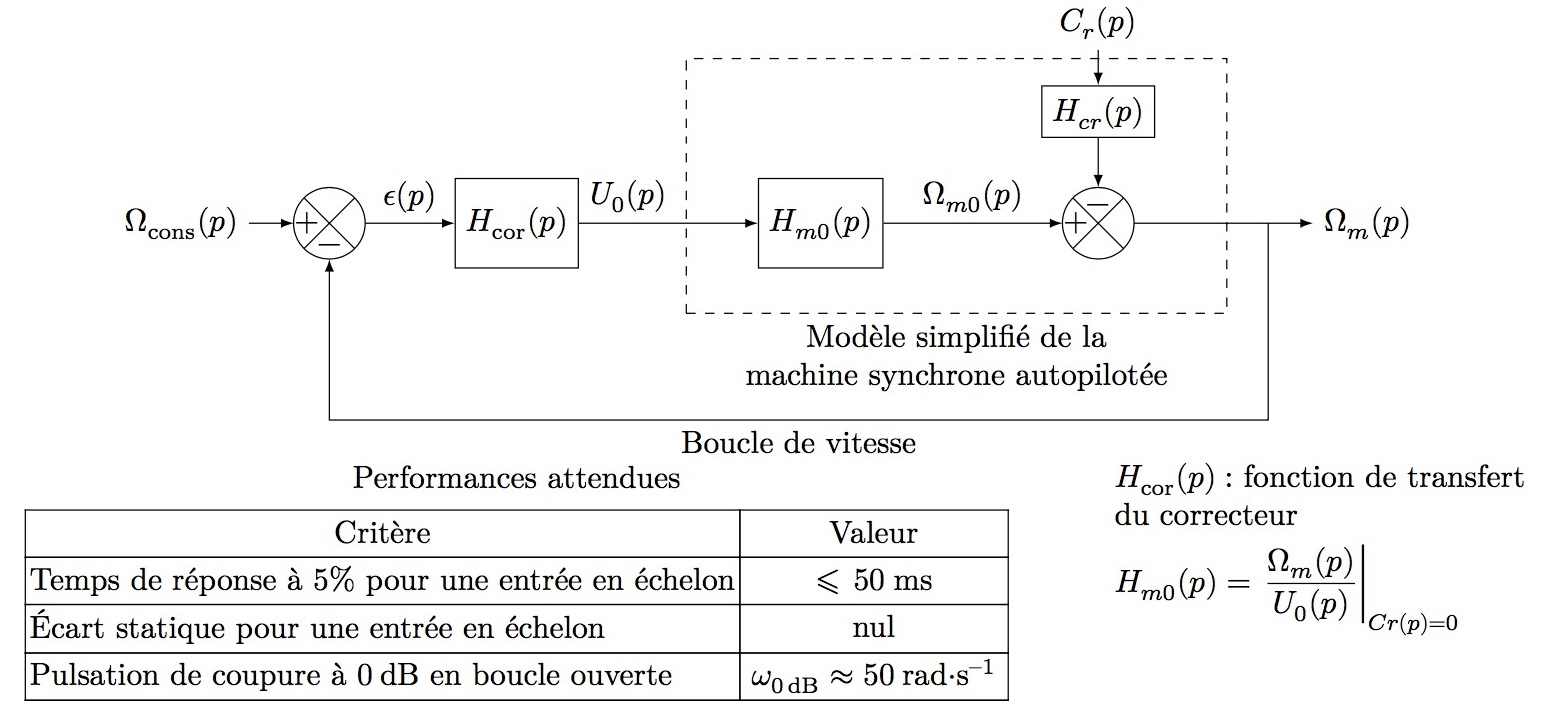
\includegraphics[width=0.9\linewidth]{img/figure_16}
 \caption{Modèle linéarisé de l'asservissement en vitesse de la machine synchrone autopilotée}
 \label{img16}
\end{figure}

\section{Synthèse}

Le correcteur dimensionné précédemment a été implanté dans le modèle de la figure \ref{img15} ainsi qu'un modèle
réaliste du couple de frottement $C_0$. Une simulation numérique de l'une des chaines d'asservissement a permis d'obtenir l'évolution de la vitesse d'un des moteurs du simulateur
de vol dans le cas d'une consigne de tangage analogue à celle mesurée sur la figure \ref{img15} et pour les paramètres du variateur de vitesse réglés par le constructeur. Les résultats de la simulation sont donnés sur la figure \ref{img17}.

\begin{figure}[!h]
 \centering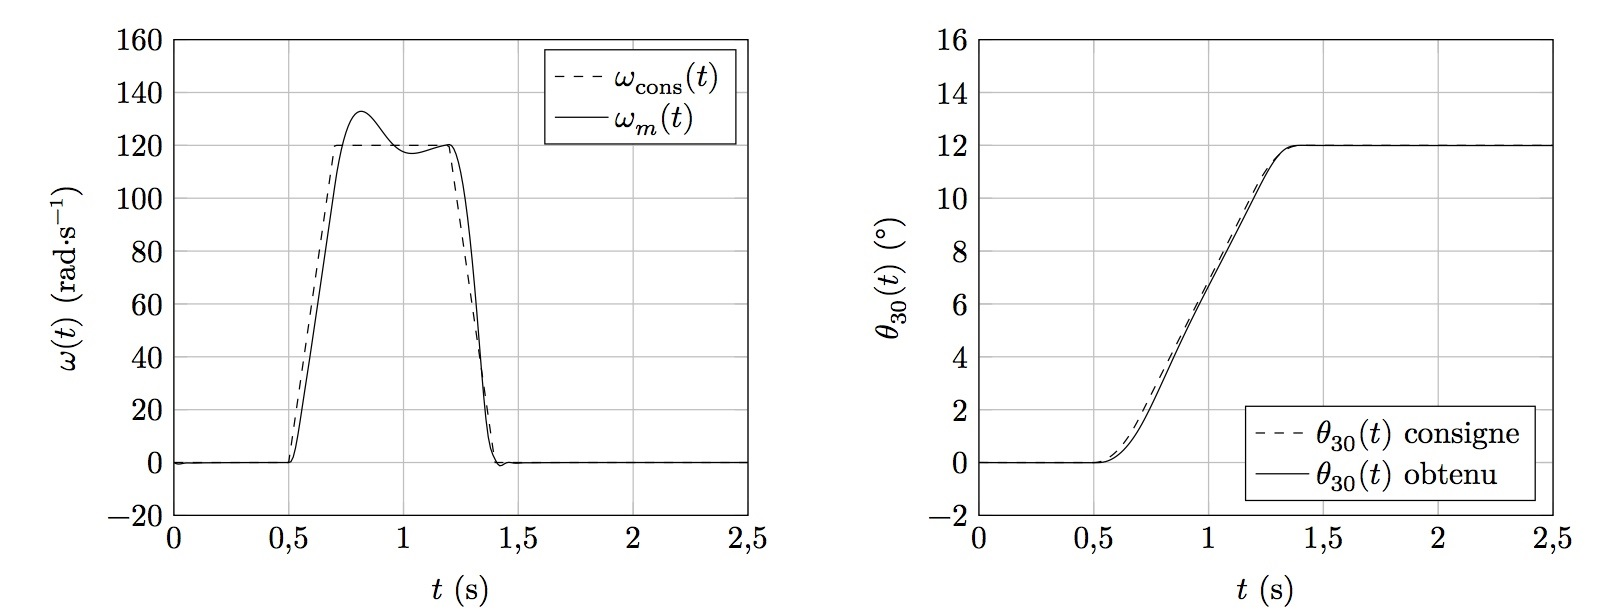
\includegraphics[width=0.7\linewidth]{img/figure_17}
 \caption{Consigne en trapèze de vitesse et réponse du modèle de l'asservissement de vitesse optimisé des
servomoteurs du simulateur de vol}
 \label{img17}
\end{figure}

\question{En s'appuyant sur la figure \ref{img17}, conclure quant à la qualité du réglage de l'asservissement de vitesse des moteurs, sachant que la consigne correspond à celle définie à la question 21 pour des conditions sévères de vol d'un DR400 (erreur autorisée de $+/-$10 rad.s$^{-1}$).}

\section{Conception}

Une vue en coupe du moto-réducteur de la figure \ref{imgB} est donné sur la figure

\begin{figure}[!h]
 \centering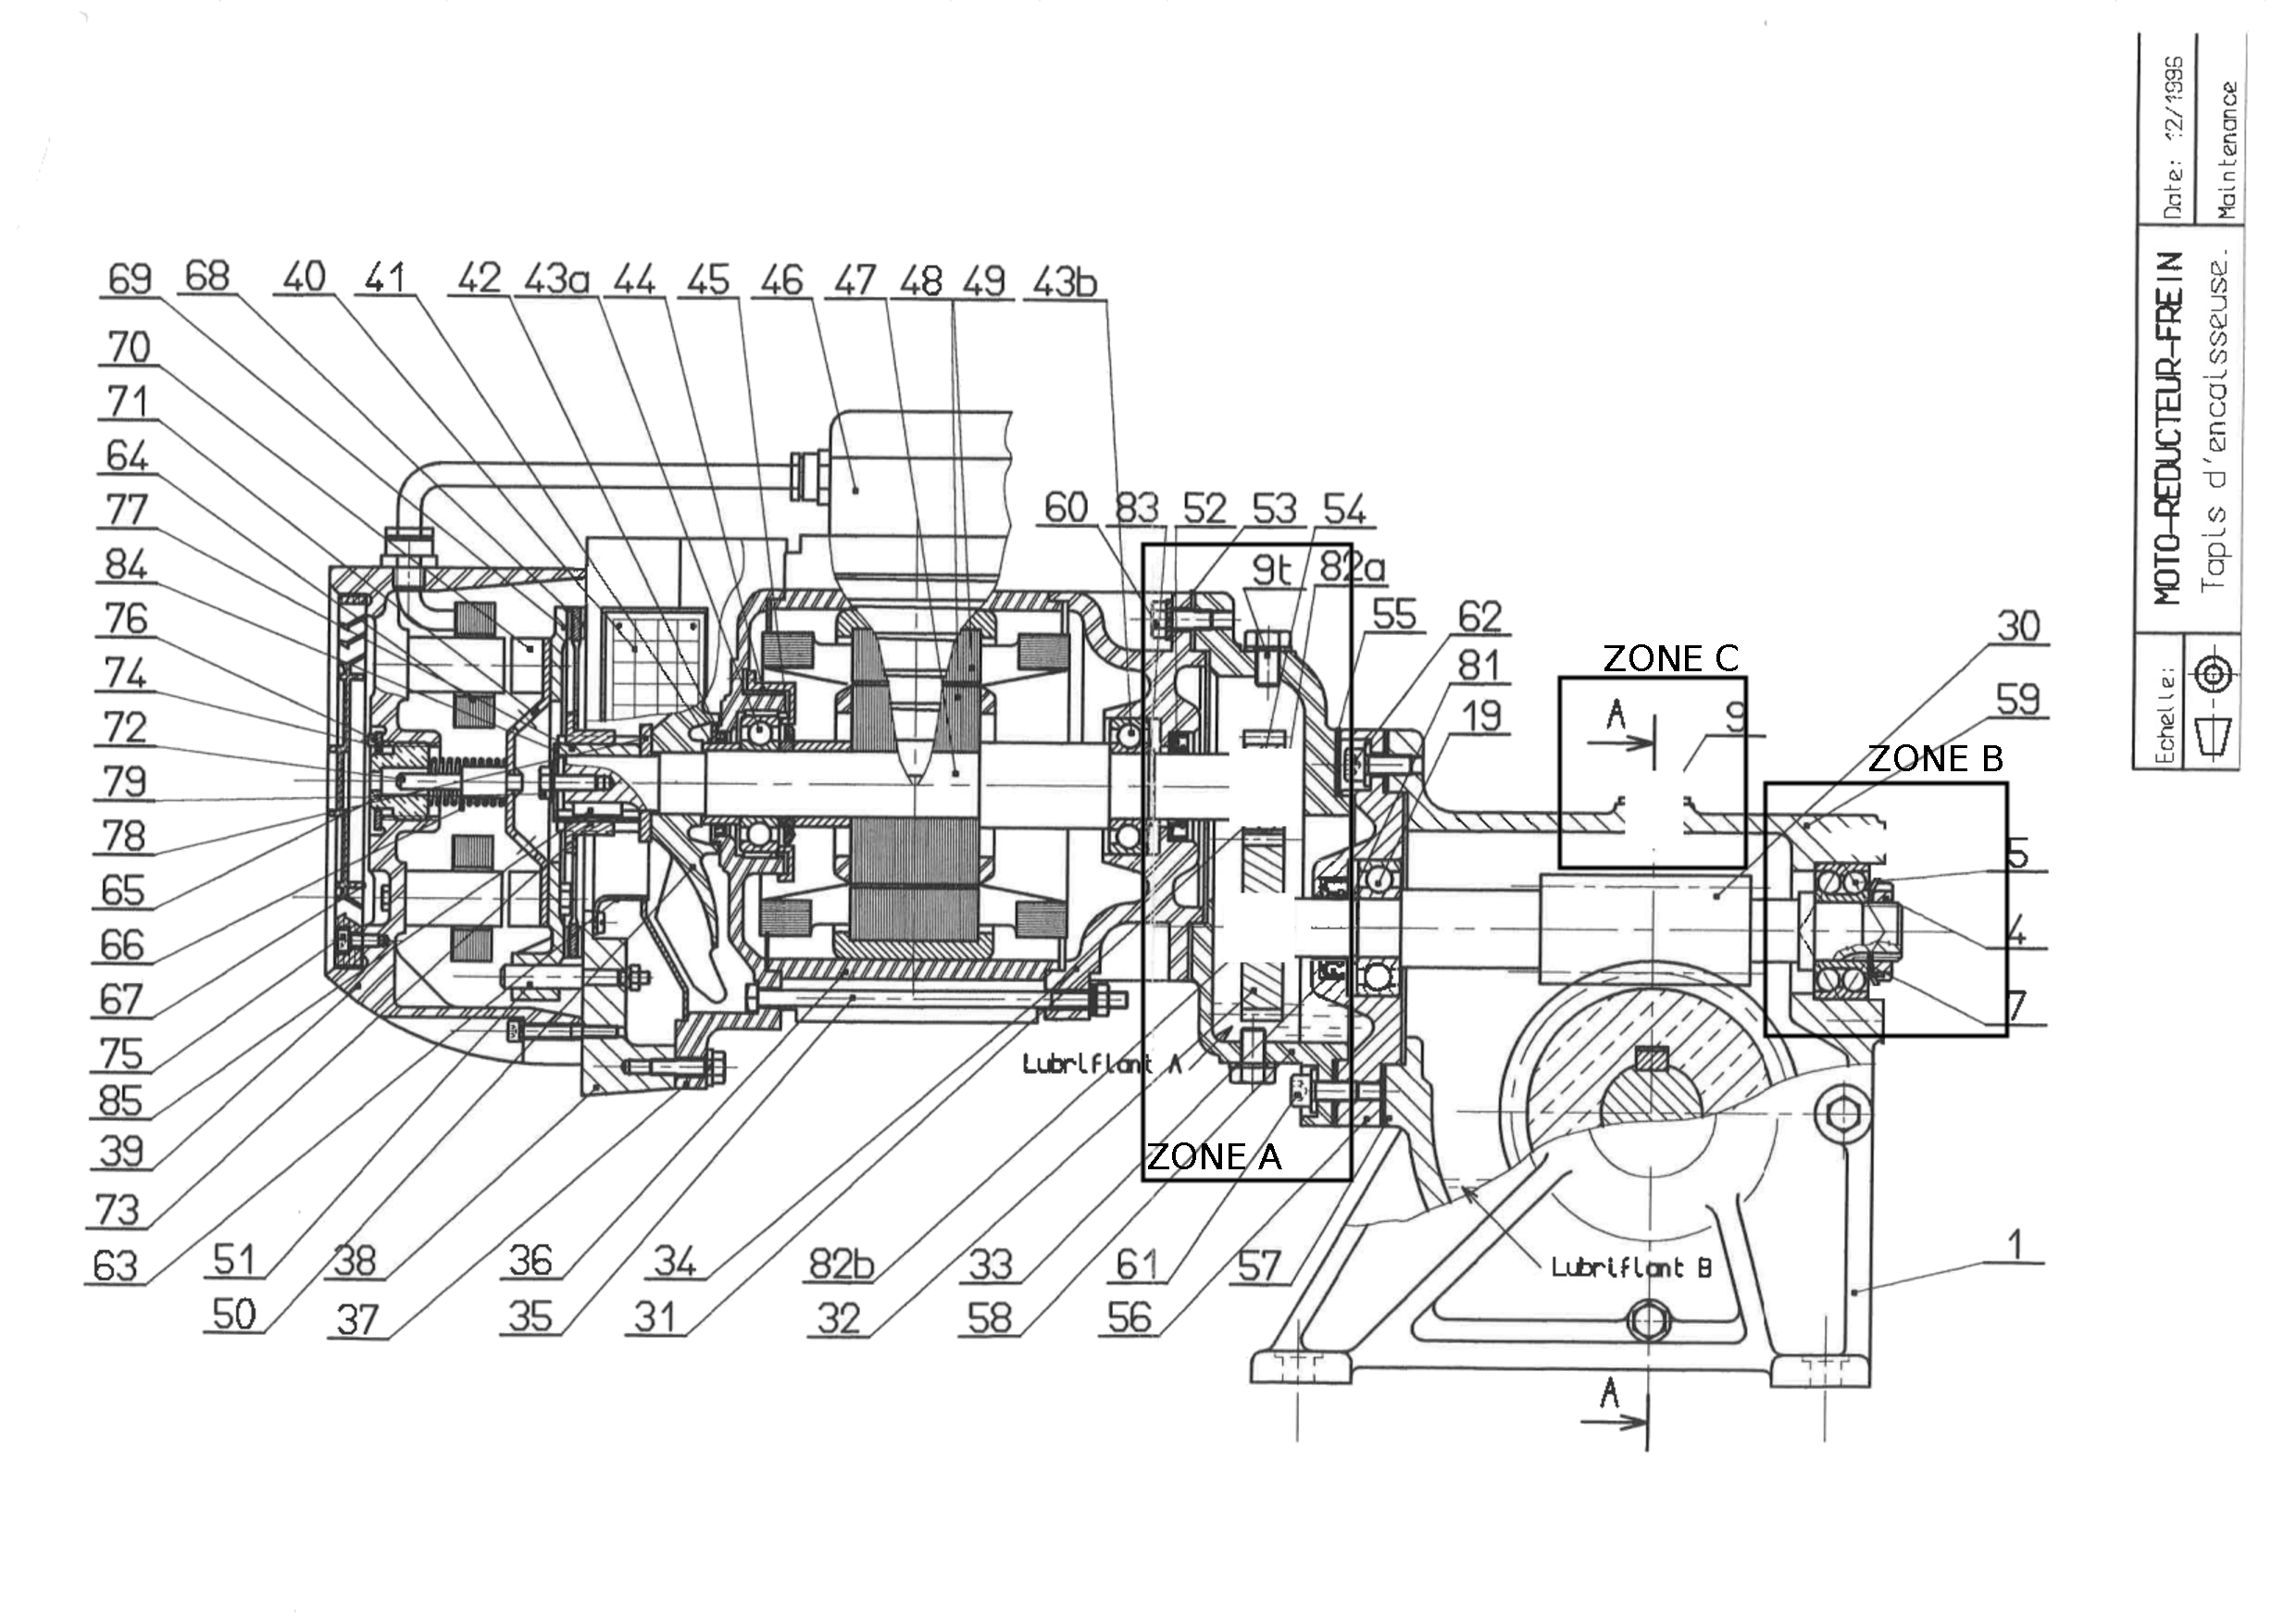
\includegraphics[width=0.7\linewidth]{img/Moto_reducteur_frein_vierge}
 \caption{Vue en coupe du motoréducteur}
 \label{img18}
\end{figure}

3 zones du mécanisme sont à compléter (à l'intérieur des cadres) sur les zoom du document réponse.

\question{Zone A (figure \ref{img_zoneA}): Compléter les liaisons encastrement entre les pignons et les axes correspondants. Il faudra utiliser des clavettes pour bloquer la rotation.}

\question{Zone B (figure \ref{img_zoneB}): Dessiner un chapeau monté en centrage court et bloqué par 3 vis dont une seule sera représentée. Le chapeau servira à empêcher le roulement à bille (5) à se décaler vers la droite.}

\question{Zone C (figure \ref{img_zoneC}): Représenter la vis bouchon de l'arrivée du lubrifiant.}

\begin{center}
----- FIN DU SUJET -----
\end{center}

\cleardoublepage

\pagestyle{documentreponse}

\section{Documents réponse}

\reponse{7}

\reponse{8}

\reponse{7}

\reponse{7}

\reponse{7}

\reponse{6}

\reponse{6}

\reponse{12}

\reponse{8}

\reponse{8}

\reponse{1}

\begin{figure}[!h]
 \centering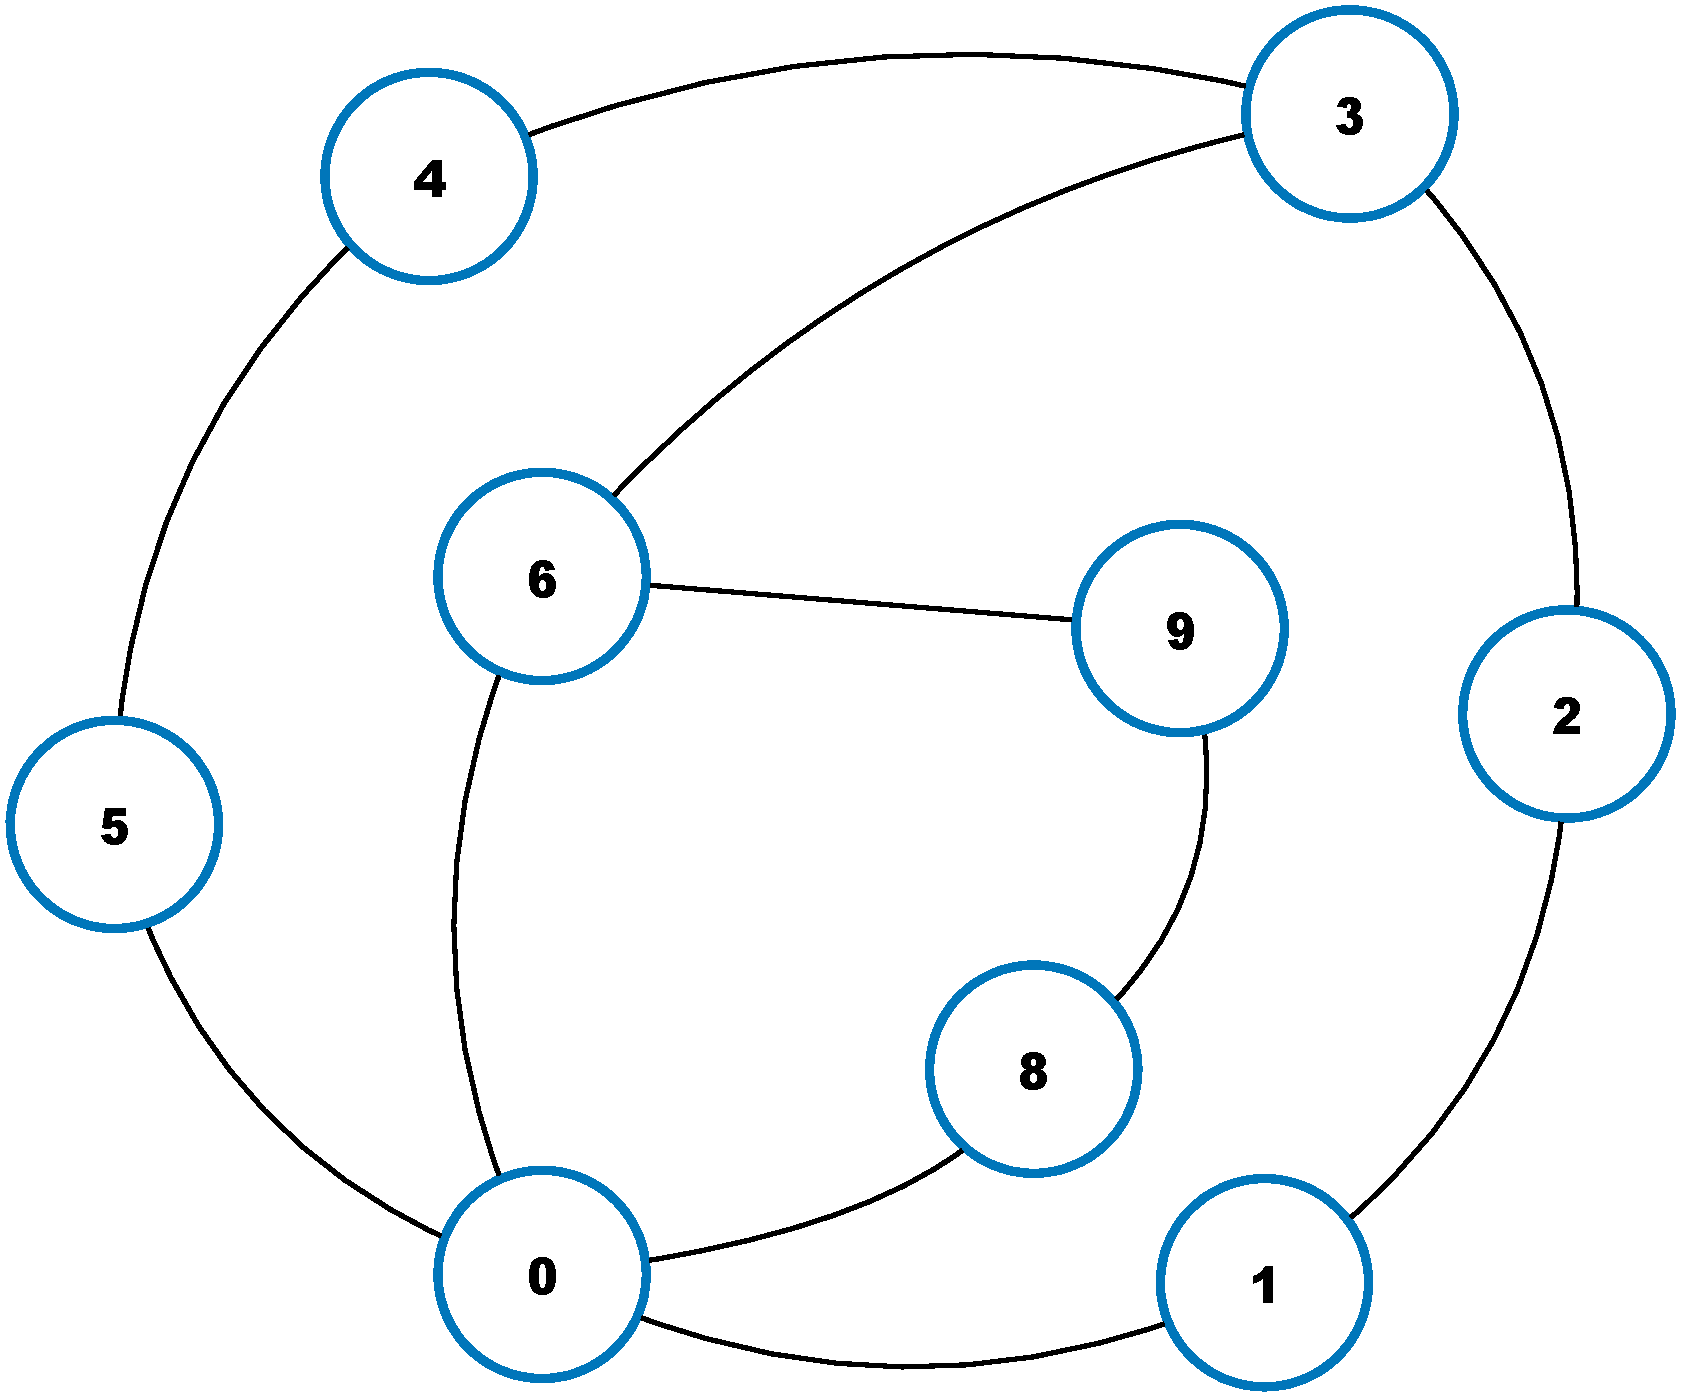
\includegraphics[width=0.4\linewidth]{img/graphe_liaisons}
 \caption{Graphe des liaisons à compléter}
 \label{imggraphe}
\end{figure}

\reponse{9}

\reponse{18}

\reponse{16}

\reponse{8}

\reponse{15}


\reponse{6}

\reponse{6}

\reponse{6}

\newpage

\reponse{1}

\begin{figure}[!h]
 \centering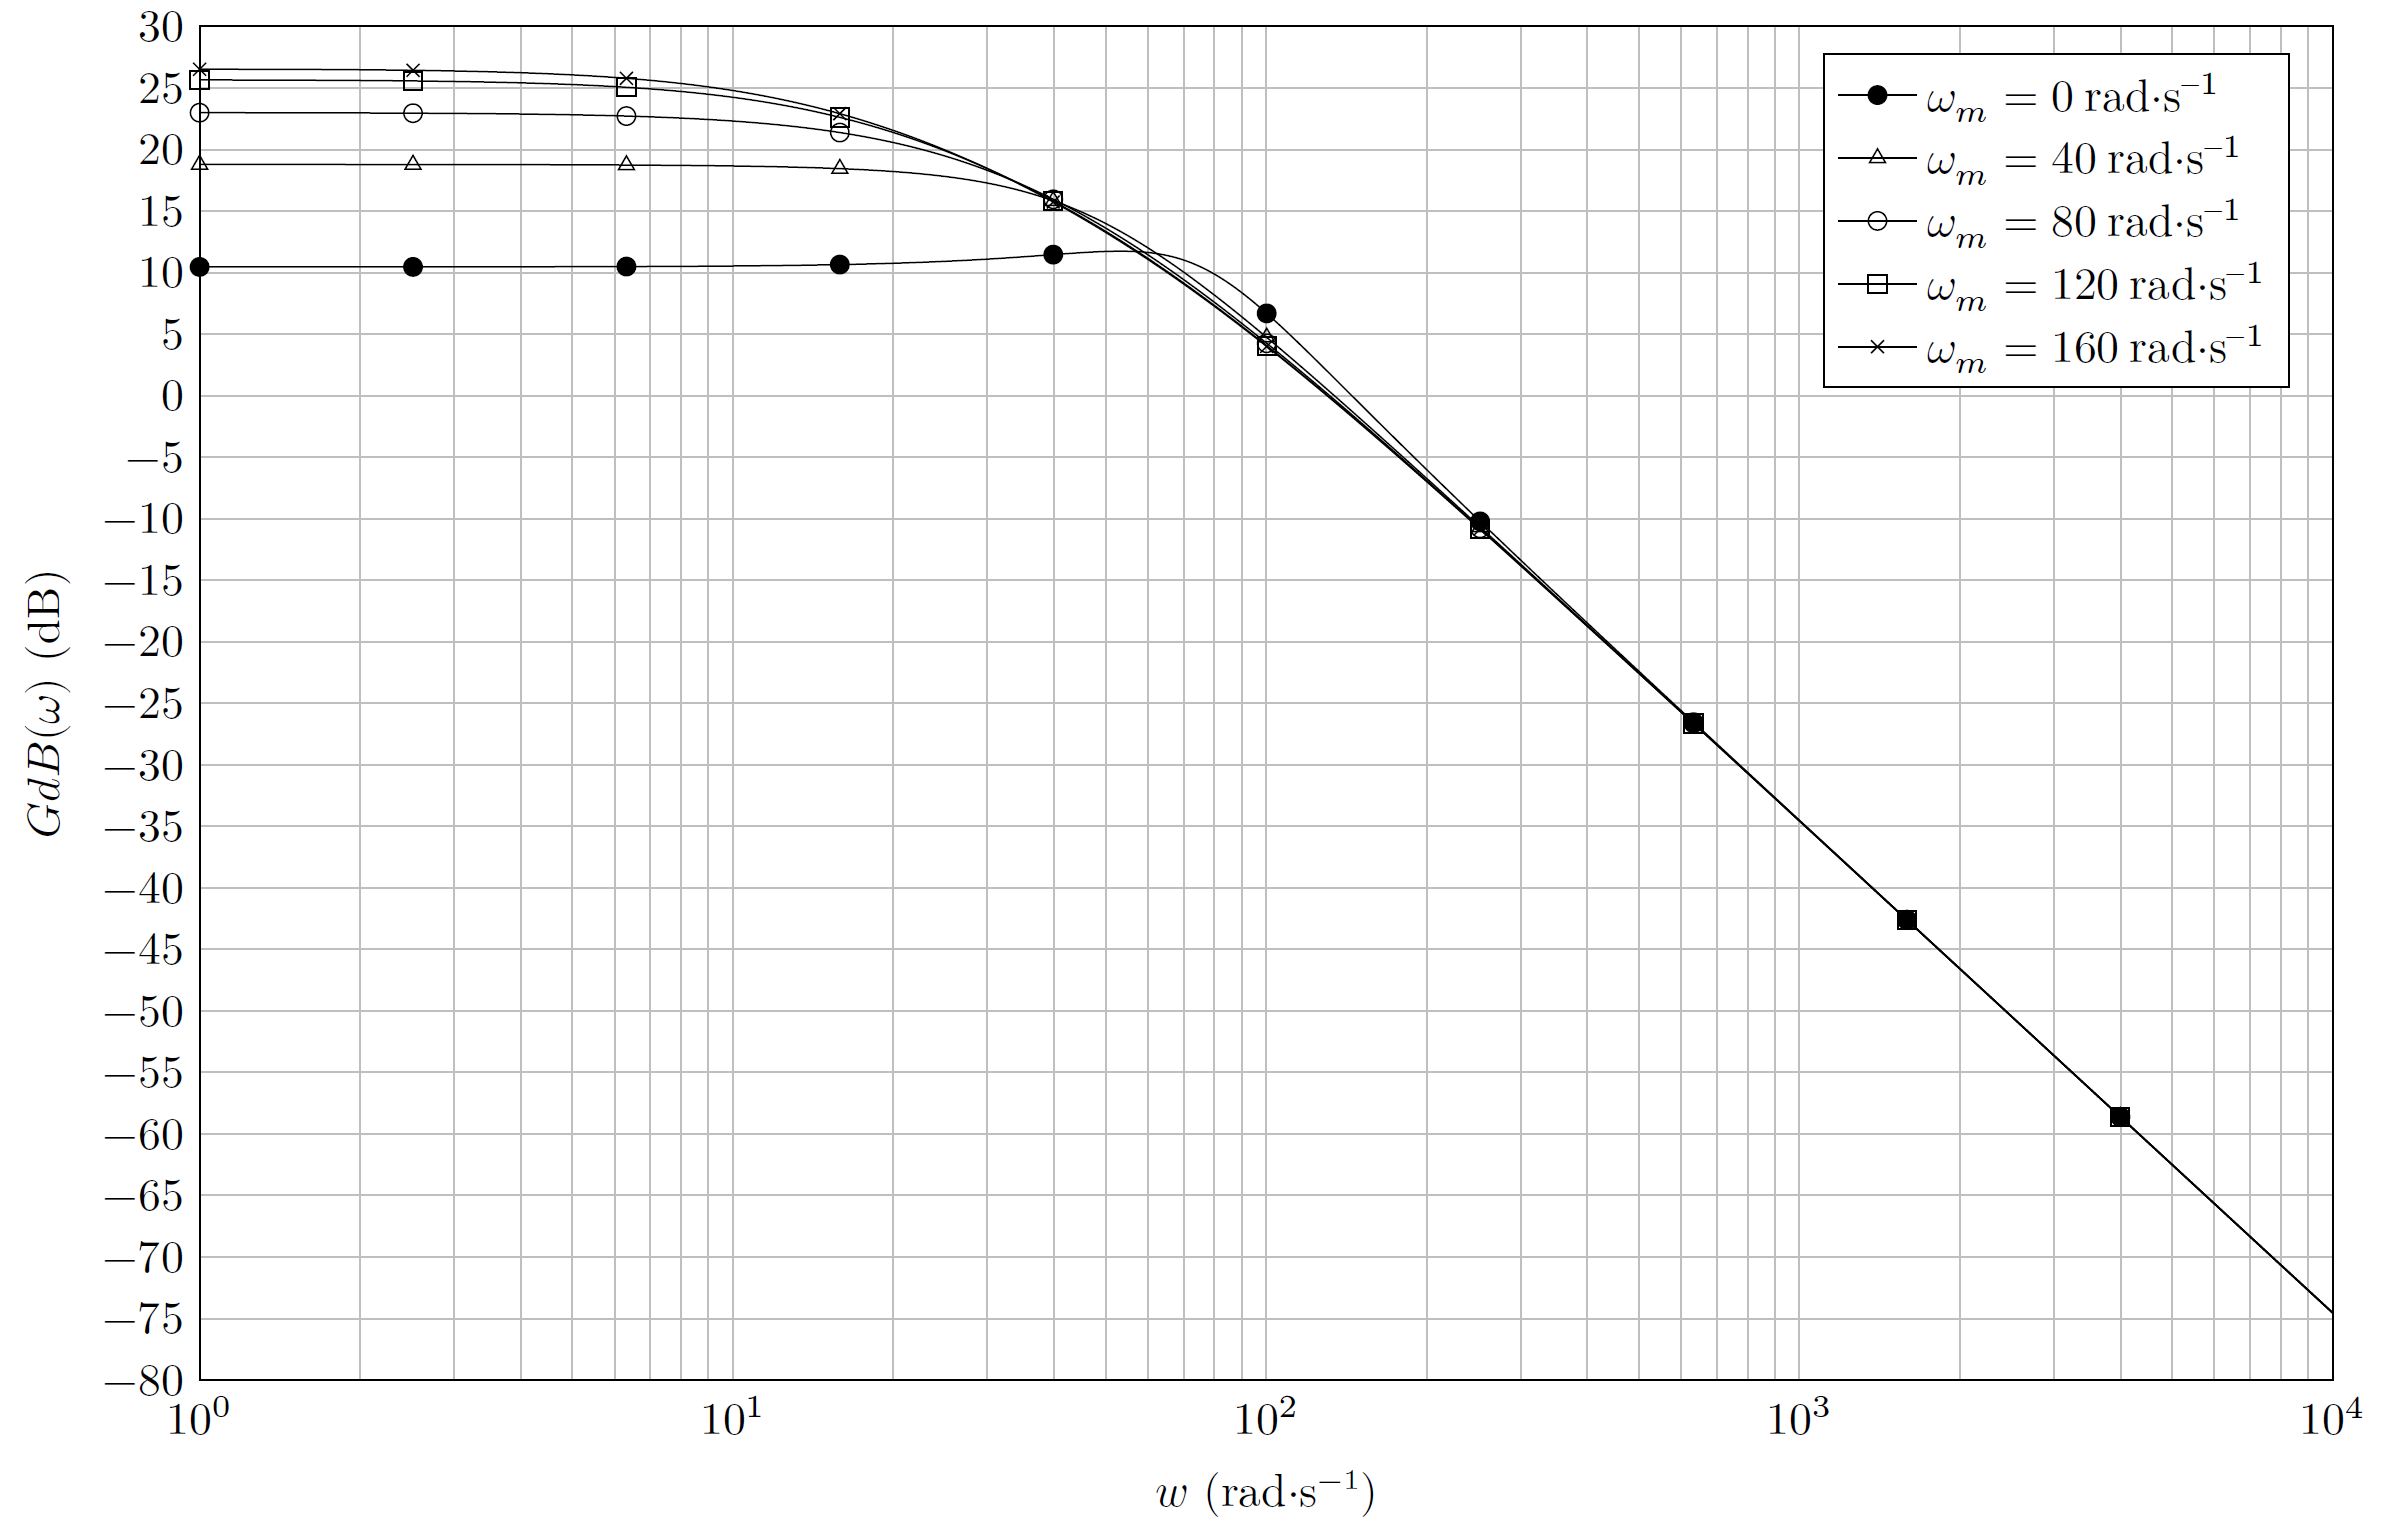
\includegraphics[width=0.7\linewidth]{img/figure_E1}\\
 \centering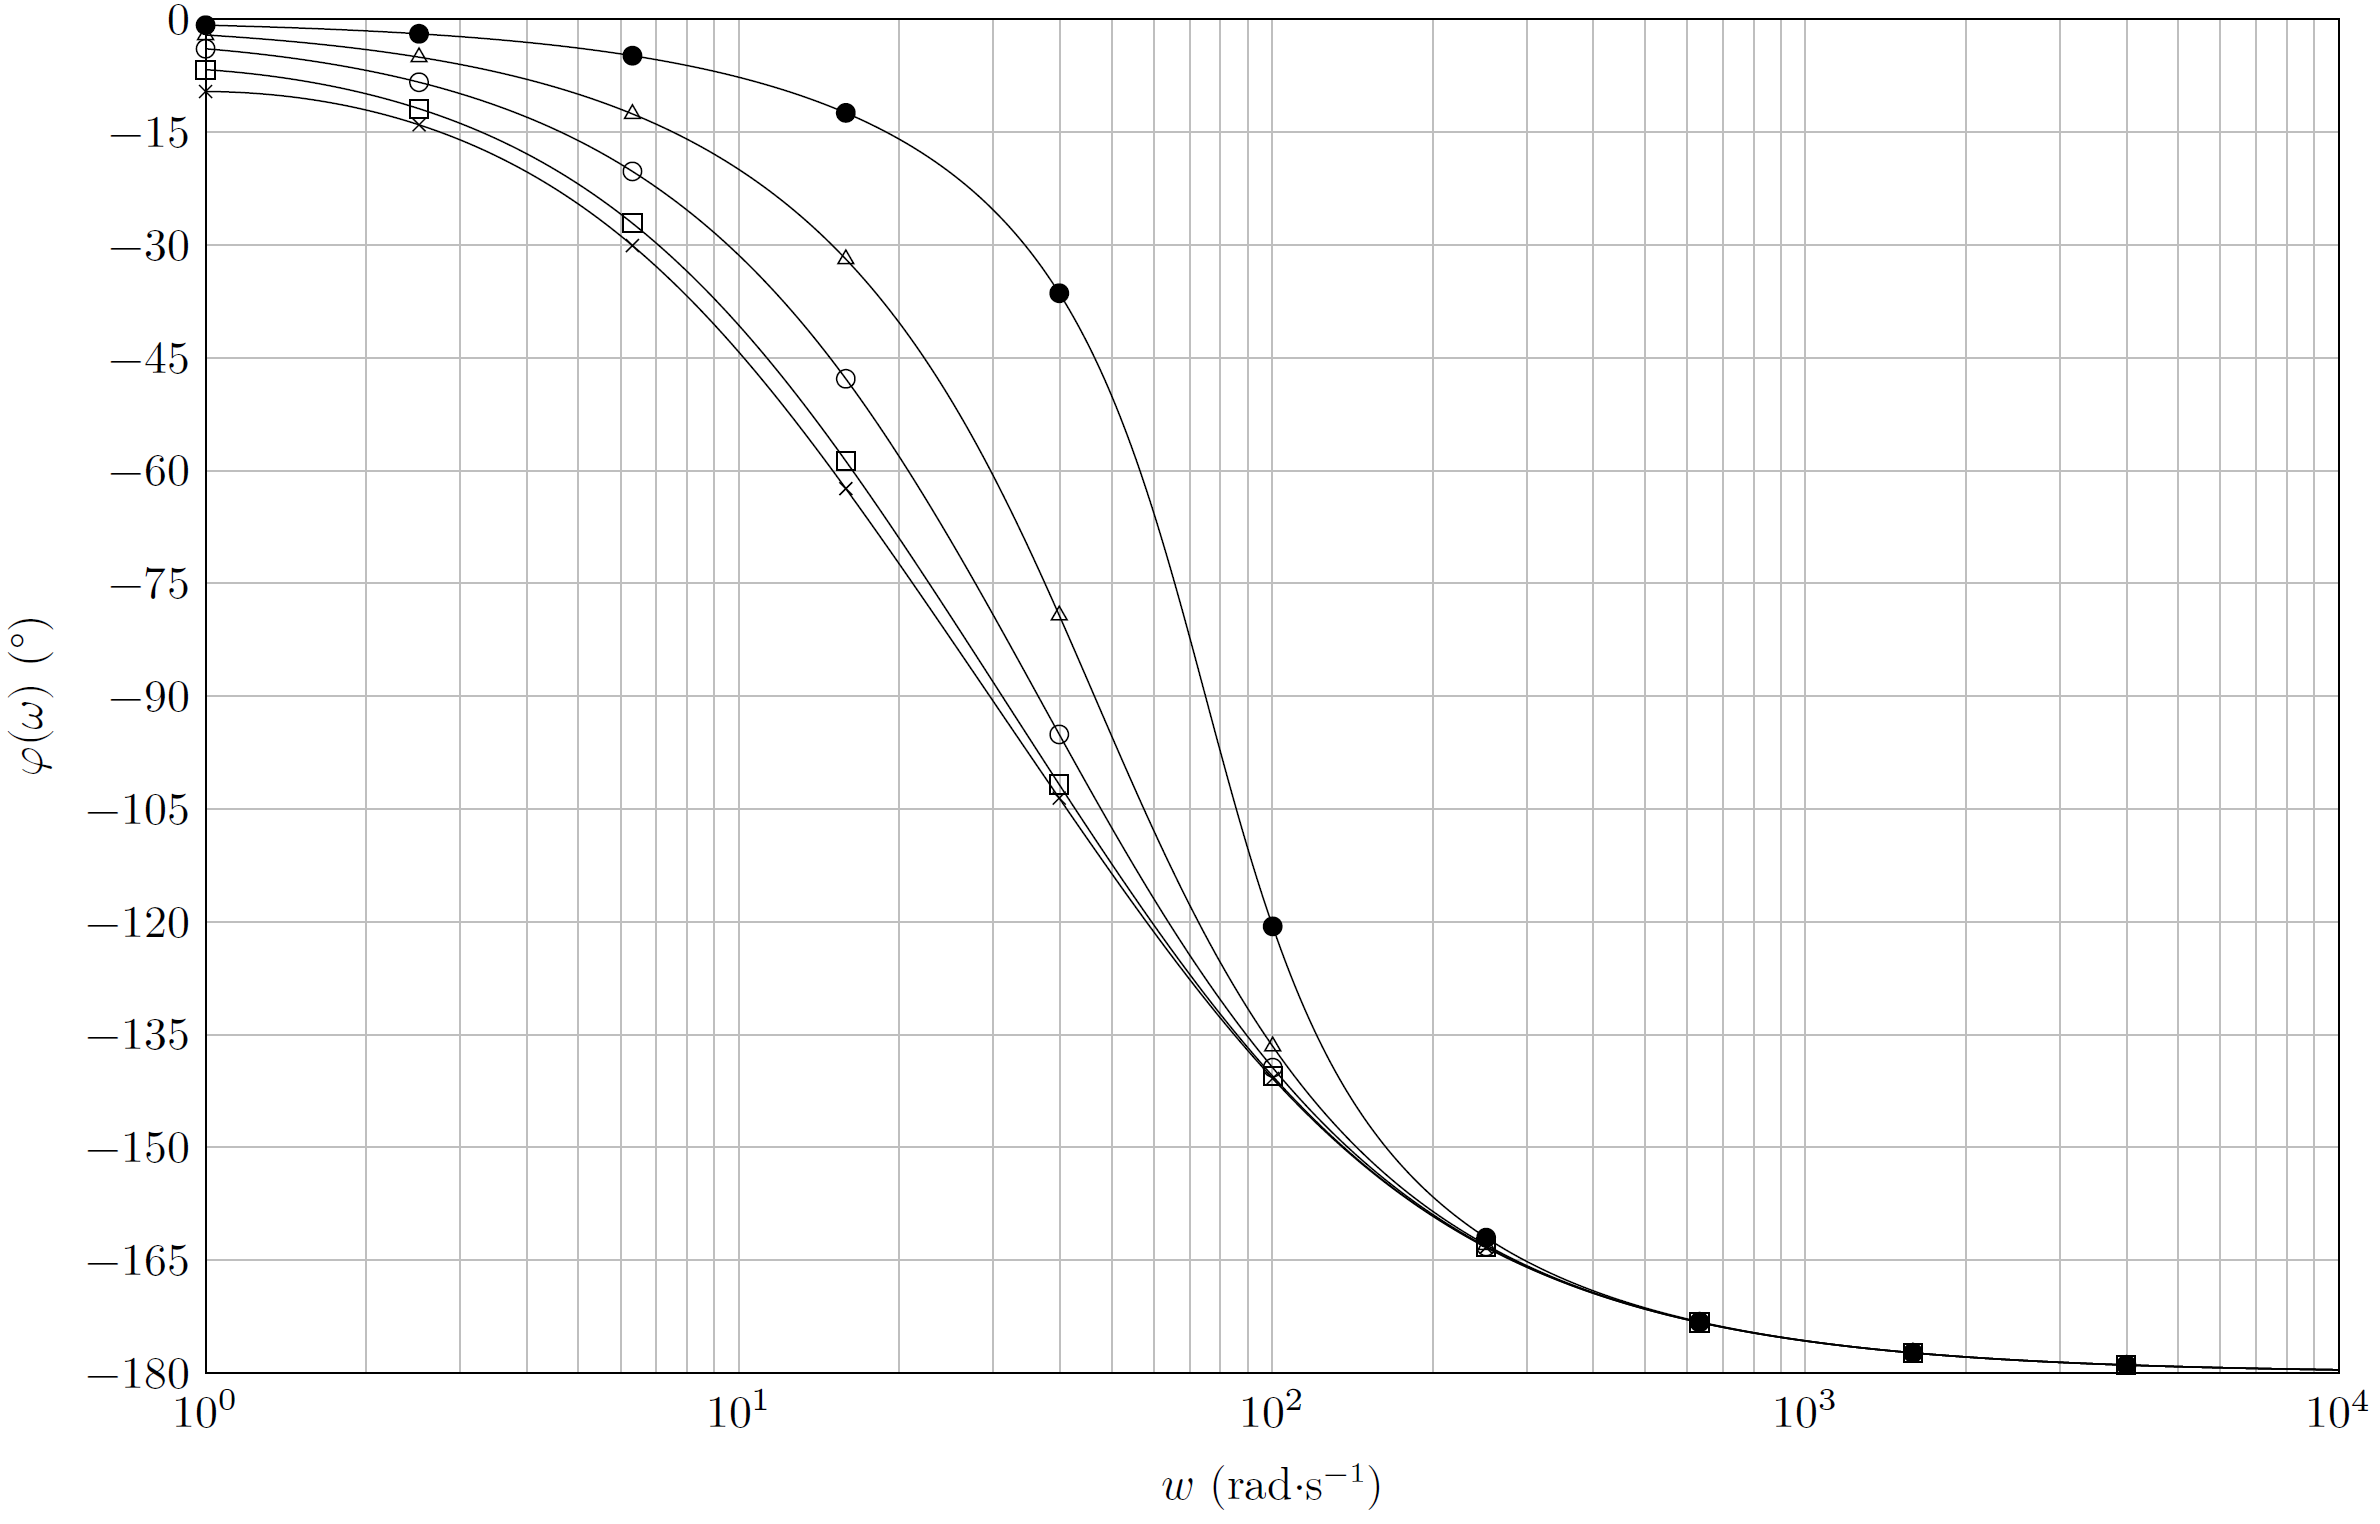
\includegraphics[width=0.7\linewidth]{img/figure_E2}
 \caption{Diagrammes de Bode du modèle de la machine synchrone autopilotée, caractérisée par la fonction de transfert complexe$\left.\frac{\Omega_m(p)}{U_0(p)}\right|_{C_r(p)=0}$ pour différentes valeurs de vitesse moteur $\omega_m$ et $C_r(p)=0$}
 \label{imgE}
\end{figure}

\newpage

\reponse{10}

\reponse{6}

\reponse{6}

\reponse{6}

\newpage

\reponse{1}

\begin{figure}[!h]
 \centering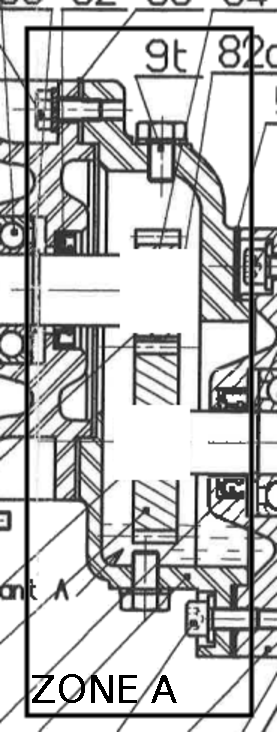
\includegraphics[width=0.35\linewidth]{img/Moto_reducteur_frein_vierge_A}
 \caption{Zone A}
 \label{img_zoneA}
\end{figure}

\newpage

\reponse{1}

\begin{figure}[!h]
 \centering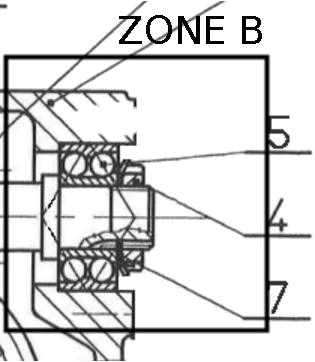
\includegraphics[width=0.4\linewidth]{img/Moto_reducteur_frein_vierge_B}
 \caption{Zone B}
 \label{img_zoneB}
\end{figure}

\reponse{1}

\begin{figure}[!h]
 \centering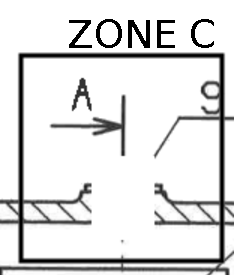
\includegraphics[width=0.4\linewidth]{img/Moto_reducteur_frein_vierge_C}
 \caption{Zone C}
 \label{img_zoneC}
\end{figure}

\ifdef{\public}{\end{document}}{}

\newpage
\cleardoublepage

\pagestyle{correction}

\setcounter{equation}{0}

\section{Correction}

\cor

\begin{itemize}
 \item Coût minimal (vol tradi): $C_{vt}=45.135+35.25=6950\euro$,
 \item Coût minimal (formule mutli-m): $C_{vt}=40.135+5.35+40.25=6575\euro$,
\end{itemize}

Ce qui correspond à une économie de $6950-6575=375\euro$, soit un peu plus de 5\%, en effet, $0,05.6950=347,5\euro$, l'exigence est respectée.

\cor

$\overrightarrow{\Omega_{3/0}}=\overrightarrow{\Omega_{3/6}}+\overrightarrow{\Omega_{6/0}}$

$\overrightarrow{\Omega_{3/0}}=\dot{\theta}_{z36}.\overrightarrow{z_6}+\dot{\theta}_{x36}.\overrightarrow{x_6}+\dot{\theta}_{60}.\overrightarrow{z_6}$

Avec: $\overrightarrow{z_6}=cos\theta_{x36}.\overrightarrow{z_3}+sin\theta_{x36}.\overrightarrow{y_3}$

donc $\overrightarrow{\Omega_{3/0}}=\left(\begin{array}{c}\dot{\theta}_{x36}\\ (\dot{\theta}_{z36}+\dot{\theta}_{60}).sin\theta_{x36} \\ (\dot{\theta}_{z36}+\dot{\theta}_{60}).cos\theta_{x36} \end{array}\right)_{(\overrightarrow{x_3},\overrightarrow{y_3},\overrightarrow{z_3})}$

\cor

Pour un tangage seul, il faut que les composantes suivant $\overrightarrow{x_3}$ et $\overrightarrow{y_3}$ soient nulles, soit 

$\dot{\theta}_{x36}=0$, donc $\theta_{x36}$=cste et $(\dot{\theta}_{z36}+\dot{\theta}_{60}).sin\theta_{x36}=0$, donc $\theta_{x36}=0$.

\cor

$\overrightarrow{OA}+\overrightarrow{AB}+\overrightarrow{BC}+\overrightarrow{CE}+\overrightarrow{EO}=\overrightarrow{0}$

$r.\overrightarrow{x_1}+l.\overrightarrow{y_2}-d_{32}.\overrightarrow{x_3}-h_3.\overrightarrow{y_3}-L.\overrightarrow{x_6}+d_{02}.\overrightarrow{x_0}-h_{01}.\overrightarrow{y_0}=\overrightarrow{0}$

\cor

Sur $\overrightarrow{x_0}$:

$r.cos\theta_{10}-l.sin\theta_{20}-d_{32}.cos\theta_{30}+h_3.sin\theta_{30}-L.cos\theta_{60}+d_{02}=0$

Sur $\overrightarrow{y_0}$:

$r.sin\theta_{10}+l.cos\theta_{20}-d_{32}.sin\theta_{30}-h_3.cos\theta_{30}-L.sin\theta_{60}-h_{01}=0$

\cor

$\overrightarrow{HI}+\overrightarrow{ID}+\overrightarrow{DC}+\overrightarrow{CE}+\overrightarrow{EH}=\overrightarrow{0}$

$r.\overrightarrow{x_5}+l.\overrightarrow{y_4}+d_{31}.\overrightarrow{x_3}-h_3.\overrightarrow{y_3}-L.\overrightarrow{x_6}+d_{01}.\overrightarrow{x_0}-h_{01}.\overrightarrow{y_0}=\overrightarrow{0}$

\cor

Sur $\overrightarrow{x_0}$:

$r.cos\theta_{50}-l.sin\theta_{40}+d_{31}.cos\theta_{30}+h_3.sin\theta_{30}-L.cos\theta_{60}+d_{01}=0$

Sur $\overrightarrow{y_0}$:

$r.sin\theta_{50}+l.cos\theta_{40}+d_{31}.sin\theta_{30}-h_3.cos\theta_{30}-L.sin\theta_{60}-h_{01}=0$

\cor

$r.(cos\theta_{50}-cos\theta_{10})-l.(sin\theta_{40}-sin\theta_{20})+cos\theta_{30}.(d_{31}+d_{32})+d_{01}-d_{02}=0$

or $d=d_{32}+d_{31}=d_{02}-d_{01}$

$r.(cos\theta_{50}-cos\theta_{10})-l.(sin\theta_{40}-sin\theta_{20})+(d_{31}+d_{32}).(cos\theta_{30}.-1)=0$

$r.(sin\theta_{50}-sin\theta_{10})+l.(cos\theta_{40}-cos\theta_{20})+sin\theta_{30}.(d_{31}+d_{32})=0$

\cor

On a alors: $\lambda_1=r$, $\lambda_2=l$, $\lambda_3=d$.

\cor

Avec la dernière équation de la question 8, si $\theta_{50}\simeq\theta_{10}$ et $\theta_{40}\simeq \theta_{20}$, alors :

$-2.r.sin\theta_{10}+d.sin\theta_{30}=0$, donc $\theta_{30}=arcsin\left(\frac{2.r.sin\theta_{10}}{d}\right)$

\cor

\begin{figure}[!h]
	\centering 
	\begin{overpic}[width=0.7\textwidth]{img/graphe_liaisons}
 	\put (88,15) {Pivot(A,$\overrightarrow{z_0}$)}
  	\put (92,62) {Pivot(B,$\overrightarrow{z_0}$)}
   	\put (57,65) {Pivot(C,$\overrightarrow{z_0}$)}
    \put (50,83) {Pivot(D,$\overrightarrow{z_0}$)}
    \put (30,32) {Pivot(E,$\overrightarrow{z_0}$)}
    \put (45,50) {Pivot(F,$\overrightarrow{z_0}$)}
    \put (0,12) {Pivot(H,$\overrightarrow{z_0}$)}
    \put (-5,55) {Pivot(I,$\overrightarrow{z_0}$)}
    \put (45,-2) {Pivot(O,$\overrightarrow{z_0}$)}
    \put (72,30) {Glissière($\overrightarrow{y_6}$)}
    \put (38,13) {Pivot(J,$\overrightarrow{z_0}$)}
	\end{overpic}
\end{figure}

\cor

Méthode statique:
\begin{itemize}
 \item $r_s=6.(9-1)-2=46$,
 \item $N_s=10.5+5.1=55$,
 \item $h=9$.
\end{itemize}

Méthode cinématique:
\begin{itemize}
 \item 3 cycles indépendants et $m=2$,
 \item $N_c=10.1+1.1=11$,
 \item $h=6.3-11+2=9$.
\end{itemize}

\cor

$\left\{V_{8/0}\right\}=\left\{\begin{array}{c c}0 & 0 \\ 0 & 0 \\ \omega_{z80} & 0 \end{array}\right\}_{(J,\overrightarrow{x_0},\overrightarrow{y_0},\overrightarrow{z_0})}=\left\{\begin{array}{c c}0 & -h_{02}.\omega_{z80} \\ 0 & -d_{03}.\omega_{z80} \\ \omega_{z80} & 0\end{array}\right\}_{(E,\overrightarrow{x_0},\overrightarrow{y_0},\overrightarrow{z_0})}$, 
$\left\{V_{8/9}\right\}=\left\{\begin{array}{c c}0 & 0 \\ 0 & V_{J,y89} \\ 0 & 0\end{array}\right\}_{(J/E,\overrightarrow{x_0},\overrightarrow{y_0},\overrightarrow{z_0})}$

$\left\{V_{9/6}\right\}=\left\{\begin{array}{c c}0 & 0 \\ 0 & 0 \\ \omega_{z96} & 0\end{array}\right\}_{(F,\overrightarrow{x_0},\overrightarrow{y_0},\overrightarrow{z_0})}=\left\{\begin{array}{c c}0 & -h_6.\omega_{z96} \\ 0 & -d_{61}.\omega_{z96} \\ \omega_{z96} & 0\end{array}\right\}_{(E,\overrightarrow{x_0},\overrightarrow{y_0},\overrightarrow{z_0})}$, 
$\left\{V_{6/0}\right\}=\left\{\begin{array}{c c}0 & 0 \\ 0 & 0 \\ \omega_{z60} & 0\end{array}\right\}_{(B,\overrightarrow{x_0},\overrightarrow{y_0},\overrightarrow{z_0})}$

\cor

$\left\{V_{8/0}\right\}=\left\{V_{8/9}\right\}+\left\{V_{9/6}\right\}+\left\{V_{6/0}\right\}$

$\left\{\begin{array}{l}
0=0+0+0 \\
0=0+0+0 \\
\omega_{z80}=0+\omega_{z96}+\omega_{z60} \\
-h_{02}.\omega_{z80}=-sin\theta_{80}.V_{J,y89}+\omega_{z96}.(-h_6.cos\theta_{60}+d_{61}.sin\theta_{60}) \\
-d_{03}.\omega_{z80}=cos\theta_{80}.V_{J,y89}+\omega_{z96}.(-h_6.sin\theta_{60}-d_{61}.cos\theta_{60}) \\
0=0+0+0
\end{array}\right.$

\cor

On a trois équations qui ne nous apportent aucune information ($0=0$), on a donc $h=3$.

\cor

En remplaçant une pivot par une pivot glissant et une par une rotule (cela peut être la même auquel cas cela devient une linéaire annulaire), on obtient un système isostatique avec les mêmes mobilités.

\cor


pour t $\in[0,t_1]$, $\omega_m=\frac{\omega_{max}}{t_1}.t$, donc 
$\theta_m=\frac{1}{2}.\frac{\omega_{max}}{t_1}.t^2$

pour t $\in[t_1,t_2]$, $\omega_m=\omega_{max}$, donc 
$\theta_m=\omega_{max}.\left(t-\frac{1}{2}.t_1\right)$

pour t $\in[t_2,t_3]$, $\omega_m=\frac{\omega_{max}}{t_2-t_3}.(t-t_3)$, donc 
$\theta_m=\frac{\omega_{max}}{t_2-t_3}.\left(\frac{1}{2}.t^2-t_3.t+\frac{1}{2}.\left(t_2^2-t_1.t_2+t_1.t_3\right)\right)$

\cor

Il s'agit d'un second ordre car il y a une tangente à l'origine et la phase part de 0° et arrive à -180°.

\cor

$H_{M0}(j.\omega_0)=\frac{K}{1+\frac{2.z}{\omega_0}.j.\omega_0+\frac{1}{\omega_0^2}.(j.\omega_0)^2}=\frac{K}{2.z.j}=\frac{-K}{2.z}.j$, donc $|H_{M0}(j.\omega_0)|=\frac{K}{2.z}$

\cor

$G_{dB}(\omega_0)=20.log(|H_{M0}(j.\omega_0)|)=20.logK-20.log(2.z)$

\cor

$\omega_m=120rad.s^{-1}$, donc, d'après les tracés,

$20.logK=25$, donc $K=10^{\frac{5}{4}}\simeq10.\sqrt{\sqrt{9}}\simeq10.\sqrt{3}\simeq17.5$

$G_{dB}(\omega_0)=20.logK-20.log(2.z)=18$, donc $20.log(2.z)=7$, donc $z=\frac{10^{\frac{7}{20}}}{2}\simeq\frac{10^{\frac{1}{3}}}{2} \simeq 1$

$\omega_0=30rad.s^{-1}$

\cor

$\frac{\Omega_m(p)}{\Omega_{cons}(p)}=\frac{H_{m0}(p)}{1+H_{m0}(p)}=\frac{K}{1+\frac{2.z}{\omega_0}.p+\frac{p^2}{\omega_0^2}+K}=\frac{\frac{K}{K+1}}{1+\frac{2.z}{(K+1).\omega_0}.p+\frac{p^2}{(K+1).\omega_0^2}+K}\simeq \frac{0.95}{1+\frac{p}{177,5}+\frac{p^2}{16650}}$

\cor

$e_s=\lim\limits_{p\to 0}p.\epsilon(p)=\lim\limits_{p\to 0}p.\Omega_{cons}.\left(1-\frac{H_{m0}(p)}{1+H_{m0}(p)}\right)=\lim\limits_{p\to 0}p.\frac{1}{p}.\left(1-\frac{K}{1+K}\right)=\frac{1}{1+K}$, donc l'écart statique n'est nul, cela ne répond pas au cahier des charges.

\cor

La figure \ref{img17} montre un dépassement de 10 $rad.s^{-1}$ environ par rapport à la vitesse consigne(erreur autorisée). La figure \ref{img17} montre également une vitesse max de consigne de 120 $rad.s^{-1}$ (définie à la question 21). Le réglage semble donc cohérent avec les attendus lors d'une phase de vol en conditions sévères.

\newpage

\cor

\begin{figure}[!h]
 \centering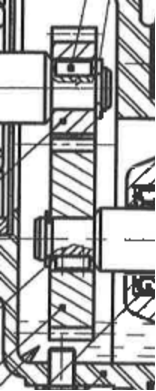
\includegraphics[width=0.35\linewidth]{img/Moto_reducteur_frein_A}
 \caption{Zone A}
 \label{img_zoneA_cor}
\end{figure}

\newpage

\cor

\begin{figure}[!h]
 \centering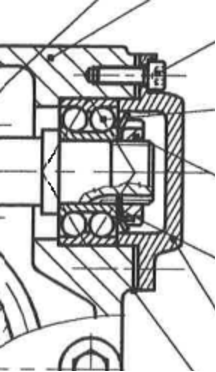
\includegraphics[width=0.4\linewidth]{img/Moto_reducteur_frein_B}
 \caption{Zone B}
 \label{img_zoneB_cor}
\end{figure}

\cor

\begin{figure}[!h]
 \centering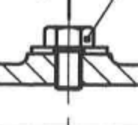
\includegraphics[width=0.4\linewidth]{img/Moto_reducteur_frein_C}
 \caption{Zone C}
 \label{img_zoneC_cor}
\end{figure}


\end{document}

